%% work notes for c language, 2018/09/22
%% thesis.tex 2014/04/11
\documentclass{ucbthesis}
\usepackage[backend=bibtex,citestyle=authoryear-icomp,bibstyle=authoryear,maxbibnames=9]{biblatex}
\setlength{\bibitemsep}{.4\baselineskip}
\addbibresource{../mendeley_bibtex.bib}
\addbibresource{../style/mendeley_bibtex_edited.bib}
\addbibresource{../manual_additions.bib}
\usepackage{indentfirst}
\usepackage[usenames,dvipsnames]{xcolor}
\usepackage[pdftex]{graphicx}
\usepackage{amsmath}
\usepackage{amssymb}
\usepackage{amsthm}
\usepackage{algorithm2e}
\usepackage{booktabs}
\setlength{\extrarowheight}{.33\baselineskip}
\usepackage{url}
\usepackage{titlesec}
\usepackage{float}
\usepackage{subcaption}
\usepackage{enumitem}
\usepackage{multirow}
\usepackage{paragraph-marginals}
\usepackage{tabularx}
\usepackage{array}
\usepackage{rotating}
\usepackage{enumerate}
\usepackage[colorlinks]{hyperref}
\hypersetup{
  citecolor=Cerulean,
  urlcolor=Cerulean
}

% Prevent page breaks in the middle of paragraphs.
\widowpenalties 1 10000
\raggedbottom

% Format paragraphs as sections
\setcounter{tocdepth}{3}
\setcounter{secnumdepth}{3}

%% Math commands
\newtheorem{theorem}{Theorem}
\newtheorem{mydef}{Definition}
\DeclareMathOperator*{\argmin}{arg\,min}
\DeclareMathOperator*{\argmax}{arg\,max}

%% Misc commands
\def\algorithmautorefname{Algorithm}
\def\chapterautorefname{Chapter}
\def\sectionautorefname{Section}
\def\subsectionautorefname{Section}

\begin{document}
\title{Anytime Recognition of Objects and Scenes}
\author{Sergey Kazbekovich Karayev}
\degreesemester{Fall}
\degreeyear{2014}
\degree{Doctor of Philosophy}
\chair{Professor Trevor Darrell}
\othermembers{
Professor Ken Goldberg\\
Professor Pieter Abbeel\\
Dr Mario Fritz
}
\numberofmembers{4}
\field{Computer Science}

%!TEX root=paper/paper.tex

\maketitle
% Comment out for final.
% \approvalpage
\copyrightpage
%!TEX root=paper/paper.tex
\begin{abstract}\label{sec:abstract}
Humans are capable of perceiving a scene at a glance, and obtain deeper understanding with additional time.
Computer visual recognition should be similarly robust to varying computational budgets --- a property we call Anytime recognition.
We present a general method for learning dynamic policies to optimize Anytime performance in visual recognition.
We approach this problem from the perspective of Markov Decision Processes, and use reinforcement learning techniques.
Crucially, decisions are made at test time and depend on observed data and intermediate results.
Our method is applicable to a wide variety of existing detectors and classifiers, as it learns from execution traces and requires no special knowledge of their implementation.

We first formulate a dynamic, closed-loop policy that infers the contents of the image in order to decide which single-class detector to deploy next.
We explain effective decisions for reward function definition and state-space featurization, and evaluate our method on the PASCAL VOC dataset with a novel \emph{costliness} measure, computed as the area under an Average Precision (AP) vs. Time curve.
In contrast to previous work, our method significantly diverges from predominant greedy strategies and learns to take actions with deferred values.
If execution is stopped when only half the detectors have been run, our method obtains $66\%$ better mean AP than a random ordering, and $14\%$ better performance than an intelligent baseline.

The detection actions are costly relative to the inference performed in executing our policy.
Next, we apply our approach to a setting with less costly actions: feature selection for linear classification.
We explain strategies for dealing with unobserved feature values that are necessary to effectively classify from any state in the sequential process.
We show the applicability of this system to a challenging synthetic problem and to benchmark problems in scene and object recognition.
On suitable datasets, we can additionally incorporate a semantic back-off strategy that gives maximally specific predictions for a desired level of accuracy.
Our method delivers best results on the costliness measure, and provides a new view on the time course of human visual perception.

Traditional visual recognition obtains significant advantages from the use of many features in classification.
Recently, however, a single feature learned with multi-layer convolutional networks (CNNs) has outperformed all other approaches on the main recognition datasets.
We propose Anytime-motivated methods for speeding up CNN-based detection approaches while maintaining their high accuracy: (1) a dynamic region selection method using novel quick-to-compute features; and (2) the Cascade CNN, which adds a \emph{reject} option between expensive convolutional layers and allows the network to terminate some computation early.
On the PASCAL VOC dataset, we achieve an 8x speed-up while losing no more than 10\% of the top detection performance.

Lastly, we address the problem of image style recognition, which has received little research attention despite the significant role of visual style in conveying meaning through images.
We present two novel datasets: 80K Flickr photographs annotated with curated style labels, and 85K paintings annotated with style/genre labels.
In preparation for Anytime recognition, we perform a thorough evaluation of different image features for image style prediction.
We find that features learned in a multi-layer network perform best, even when trained with object category labels.
Our large-scale learning method also results in the best published performance on an existing dataset of aesthetic ratings and photographic style annotations.
We use the learned classifiers to extend traditional tag-based image search to consider stylistic constraints, and demonstrate cross-dataset understanding of style.
\end{abstract}

\begin{frontmatter}
    %!TEX root=paper/paper.tex
\begin{dedication}
\null\vfil
\begin{center}
To my parents, Kazbek and Valeriya.
\end{center}
\vfil\null
\end{dedication}

    \newpage
    \tableofcontents
    \newpage
    \listoffigures % maybe cancel
    \newpage
    \listoftables  % maybe cancel
    \newpage
    %!TEX root=paper/paper.tex
\begin{acknowledgements}
I am fortunate to have worked with consistently amazing people during my PhD.
My advisor Trevor Darrell has always provided wise and encouraging guidance, and supported every direction that excited me.
My close collaborator and mentor Mario Fritz is responsible for too many of ``my'' ideas to count.
Regular meetings with Pieter Abbeel helped develop the reinforcement learning formulation of vision problems presented in this thesis.
Ken Goldberg, Jitendra Malik, and Bruno Olshausen provided crucial inter-disciplinary North Stars to keep in view.
Aaron Hertzmann, Holger Winnemoeller, and Aseem Agarwala introduced me to the novel recognition problem of image style, and Alyosha Efros has been tirelessly encouraging of this line of work.

The bulk of graduate school life and learning is centered on one's peers, and at Berkeley I was lucky to be among the truly best.
Yangqing Jia, Jon Barron, Adam Roberts, Trevor Owens, Hyun Oh Song, Ning Zhang, Judy Hoffman, Allie Janoch, Jon Long, Jeff Donahue, Evan Shelhamer, Georgia Gkioxari, Saurabh Gupta, Bharath Hariharan, Subhransu Maji, Sanja Fidler, Carl Henrik Ek, Brian Kulis, Kate Saenko, Mario Christoudias, Oriol Vinyals, Ross Girshick, Sergio Guadarrama, and so many others.

Last but not least, I am deeply indebted to the love and support of my parents.
This thesis is dedicated to them.
\end{acknowledgements}

\end{frontmatter}
\pagestyle{headings}

%!TEX root=paper/paper.tex
\chapter{Introduction}\label{sec:introduction}

\section{Motivation}

\PM{Perception}
It is well known that human perception is both Anytime, meaning that a scene can be described after even a short presentation, and progressive, meaning that the quality of description increases with more time.
The progressive time course of visual perception has been confirmed by multiple studies \parencite{Vanrullen-1996,Fei-Fei-Vision-2007}, with some studies providing evidence that enhancement occurs in an ontologically meaningful way.
For example, people tend to recognize something as an animal before recognizing it as a dog \parencite{Mace-PloS-2009}.
The underlying mechanisms of this behavior are not well explored, with only a few attempts made to explain the temporal dynamics --- for instance, a promising work by \cite{Hegde-Neuro-2008} has employed the framework of sequential decision processes.

\PM{Computer applications}
Meanwhile, automated visual recognition has achieved levels of performance that allow useful real-world implementation.
We focus on two problem formulations: \emph{image classification}, in which some property of the image -- such as scene type, visual style, or even object presence -- is predicted, and \emph{object detection}, in which the location and category (or identity) of all objects in a scene is predicted.
Solutions to the two problems are often linked, as classification can be a ``subroutine'' in a detection method.
State-of-the-art methods for classification and detection tend to be computationally expensive, insensitive to Anytime demands, and not progressively enhanced.

\PM{Application}
As real-world deployment of recognition methods grows, managing resource cost (power or compute time) becomes increasingly important.
For tasks such as personal robotics, it is crucial to be able to deploy varying levels of processing to different stimuli, depending on computational demands on the robot.
A hypothetical system for vision-based advertising, in which paying customers engage with the system to have their products detected in images on the internet, presents another example.
The system has different values (in terms of cost per click) and accuracies for different classes of objects, and the backlog of unprocessed images fluctuates based on demand and available server time.
A recognition strategy to maximize profit in such an environment should exploit all signals available to it, and the quality of detections should be Anytime, depending on the length of the queue (for example, lowering recall with increased queue pressure).

\PM{Visual Features \& Classification}
For most state-of-the-art classification methods, a range of features are extracted from an image instance and used to train a classifier.
Since the feature vectors are usually high-dimensional, linear classification methods are used most often.
Features are extracted at different costs, and contribute differently to decreasing classification error.
Although it can generally be said that ``the more features, the better,'' high accuracy can of course be achieved with only a small subset of features for some instances.
Additionally, different instances benefit from different subsets of features.
For example, simple binary features are sufficient to quickly detect faces \parencite{Viola-IJCV-2004} but not more varied visual objects, while the features most useful for separating landscapes from indoor scenes \parencite{Xiao-CVPR-2010} are different from those most useful for recognizing fine distinctions between bird species \parencite{Farrell-ICCV-2011}.
\autoref{fig:features} presents several common visual features.

\PM{Detection}
Detection methods tend to employ the same visual features and classifiers but apply them to many image sub-regions.
Approaches can broadly be grouped into (A) \emph{per-class, all-region}, (B) \emph{all-class, all-region}, and (C) \emph{all-class, proposed-region} methods.
State-of-the-art \emph{all-class, proposed-region} methods such as \cite{Girshick-CVPR-2014} and \emph{per-class, all-region} methods such as \cite{Felzenszwalb2010a} are considerably slow (on the order of seconds), performing an expensive computation on (respectively) a thousand to a million image windows.
To maximize early performance gains of these methods, scene and inter-object contextual cues can be exploited in two ways.
First, regions can be processed in an intelligent order, with most likely locations selected first.
Second, if detectors are applied per class, then they can be sequenced so as to maximize the chance of finding objects actually present in the image.
And even the most recent \emph{all-class, all-region}, Convolutional Neural Net (CNN)-based detection methods such as \cite{He-ECCV-2014}, which take advantage of high-performance convolutional primitives for region processing and detect for all classes simultaneously, can be sped up using our idea of cascaded classification.

\section{Our Contributions}

\PM{Costliness}
Computing all features, running all detectors, or processing all regions for all images is infeasible in a deployment sensitive to Anytime needs, as each feature brings a significant computational burden.
Yet the conventional approach to evaluating visual recognition does not consider efficiency, and evaluates performance independently across classes.
We address the problem of selecting and combining a subset of features under an Anytime cost budget (specified in terms of wall time or total power expended or another metric) and propose a new \emph{costliness} measure of performance vs. cost.

\PM{Learning a Policy}
To exploit the fact that different instances benefit from different subsets of features, our approach to feature selection is a sequential policy.
To learn the policy parameters, we formulate the problem as a Markov Decision Process (MDP) and use reinforcement learning methods.
The method does not make many assumptions about the underlying actions, which can be existing object detectors and feature-specific classifiers.
With different settings of parameters, we can learn policies ranging from \textbf{Static, Myopic}---greedy selection not relying on any observed feature values, to \textbf{Dynamic, Non-myopic}---relying on observed values and considering future actions.
The foundational machinery is laid out in \autoref{sec:det_method}.

\PM{Per-class Detection}
For \emph{per-class} detection, the actions are time-consuming detectors applied to the whole image, as well as a quick scene classifier.
We run scene context and object class detectors over the whole image sequentially, using the results of detection obtained so far to select the next actions.
Since the actions are time-consuming, we use a powerful inference mechanism to select the best next action.
In \autoref{sec:det_evaluation}, we evaluate on the PASCAL VOC dataset and obtain better performance than all baselines when there is less time available than is needed to exhaustively run all detectors.
This work was originally presented in \cite{Karayev-NIPS-2012} and all work is open source\footnote{Available at \url{https://github.com/sergeyk/timely_object_recognition}}.

\PM{Image Classification}
Classification actions are much faster than detectors, and the action-selection method accordingly needs to be fast.
Because different features can be selected for different instances, and because our system may be called upon to give an answer at any point during its execution, the feature combination method needs to be robust to a large number of different observed-feature subsets.
In \autoref{sec:clf_chapter}, we consider several value-imputation methods and present a method for learning several classifiers for different clusters of observed-feature subsets.
We first demonstrate on synthetic data that our algorithm learns to pick features most useful for the specific test instance.
We demonstrate the advantage of non-myopic over greedy, and of dynamic over static on this and the Scene-15 visual classification dataset.
Then we show results on a subset of the hierarchical ImageNet dataset, where we additionally learn to provide the most specific answers for any desired cost budget and accuracy level.
This work was originally presented in \cite{Karayev-CVPR-2014} and all work is open source\footnote{Available at \url{https://github.com/sergeyk/anytime_recognition}}.

\PM{Cascade CNN}
We additionally investigate a novel approach for speeding up a state-of-the-art CNN-based detection method, and propose a general technique for accelerating CNNs applied to class imbalanced data.
We employ the classic idea of the cascade by inserting a \emph{reject} option between expensive convolutional layers.
When a CNN processes batches of images, which is standard for many applications, the reject layers allows ``thinning'' of the batch as it progresses through the network, thus saving processing time.
This method is applicable to both \emph{all-class, proposed-region} methods such as \cite{Girshick-CVPR-2014} and \emph{all-class, all-region} methods such as \cite{He-ECCV-2014}.
We demonstrate results --- along with a variety of strong baselines -- on the former method, and show that the Cascade CNN method obtains a nearly 10x speed-up with only marginal drop in accuracy.
All work is reported in \autoref{sec:ccnn_chapter}.

\PM{Recognizing Style}
Lastly, in \autoref{sec:style_chapter} we present two novel datasets and first results for an underexplored research problem in computer vision -- recognizing visual style.
In preparation for an Anytime approach, we evaluate several different features (including CNNs) for the task, and explore content-style correlations in our datasets.
Our large-scale learning gives state-of-the-art results on an existing dataset of image quality and photographic style, and provides a strong baseline on our contributed datasets of 80K photos and 85K paintings labeled with their style and genre.
In a demonstration of cross-dataset understanding of style, we show how results of a search by content can be filtered by style.
This work was originally presented in \cite{Karayev-BMVC-2014}, and all code is open source\footnote{Available at \url{https://github.com/sergeyk/vislab}}.

\PM{Future Directions}
This thesis provides an effective foundation for Anytime visual recognition, and points the way to interesting further developments.
Our MDP-based formulation of learning a feature-selection policy is empirically effective, but heuristic in nature.
The recently developed framework of adaptive submodularity \parencite{Golovin-and-Krause-2010-JAIR} could provide theoretical near-optimality results for some policies, but developing an appropriate objective for our task is not straightforward.
We showed our Cascade CNN model to be effective for a region-based detection task -- but the model was not trained end-to-end with the threshold layers.
An even more interesting future development would add an Anytime loss layer that combines classification output from multiple levels of the network in a cost-sensitive way.
We expand on these ideas in \autoref{sec:conclusion}.

%!TEX root=paper/paper.tex
\section{Related Work}\label{sec:related_work}

Our work spans across several sub-fields of computer vision.
Here we cover the necessary background, ordered by applicability to each chapter of this thesis.

\subsection{Detection}

\PM{Features}
Classically, the best recent performance has come from detectors that use gradient-based features to represent objects as either a collection of local patches or as object-sized windows \parencite{Dalal2005,Lowe2004}.
Classifiers are then used to distinguish between featurizations of a given class and all other possible contents of an image window.
For state-of-the-art performance, the object-sized window models are augmented with parts \parencite{Felzenszwalb2010a}, and the bag-of-visual-words models employ non-linear classifiers \parencite{Vedaldi2009}.
In \autoref{sec:det_chapter}, we employ the widely used Deformable Part Model detector \parencite{Felzenszwalb2010a}.

\PM{CNNs}
Most recently, best performance is obtained not with hand-designed features but with those learned on large-scale labeled datasets such as ImageNet \parencite{Deng-CVPR-2009} by a deep convolutional neural network (CNN) such as AlexNet \parencite{Krizhevsky-NIPS-2012}.
This has prompted attempts to apply these computationally expensive methods to detection \parencite{Erhan-CVPR-2014,Sermanet-ICLR-2014}.
The \emph{R-CNN} method of \cite{Girshick-CVPR-2014} in particular is powerful but slow, requiring costly processing of many windows.
Recent work from \cite{He-ECCV-2014} (SPP-net) sustained the high performance of R-CNN while decreasing the running time by an order of magnitude.
Our work in \autoref{sec:ccnn_chapter} is evaluated in the R-CNN framework, but applies to the SPP-net method also.

\PM{Windows}
Window proposal is most often done exhaustively over the image space as a ``sliding window'', or inexhaustively with a bottom-up segmentation approach \parencite{Uijlings-IJCV-2013}.
Some approaches use ``jump windows'' (hypotheses voted on by local features) \parencite{Vedaldi2009,Vijayanarasimhan2011}, or a bounded search over the space of all possible windows \parencite{Lampert2008a}.
In all state-of-the-art systems, the window proposal step is conceptually separate from the feature extraction and classification.

\PM{Using feedback}
None of the best-performing systems treat window proposal and evaluation as a closed-loop system, with feedback from evaluation to proposal.
Some work has been done on this topic, mostly inspired by ideas from biological vision and attention research \parencite{Butko2009,Vogel2008}.
One application to the problem of visual detection picks features with maximum value of information in a Hough-voting framework \parencite{Vijayanarasimhan2010}.
Another uses nearest-neighbor lookups of image windows to sum offset vectors onto objects \parencite{Alexe2012a}.

\PM{Multi-class context}
Most detection methods train individual models for each class.
Work on inherently multi-class detection focuses largely on making detection time sublinear in the number of classes through sharing features \parencite{Torralba2007,Fan2005}.
Inter-object context has also been shown to improve detection \parencite{Torralba2004}.
A post-processing extension to detection systems uses structured prediction to incorporate multi-class context as a principled replacement for non-maximum suppression \parencite{Desai2009}.
In a standard evaluation setup, inter-object context plays a role only in post-filtering, once all detectors have been run.
In contrast, our work leverages inter-object context in the action-planning loop.

\PM{Scene context}
The most common source of context for detection is the \emph{scene} or other non-detector cues; the most common scene-level feature is the GIST \parencite{Oliva-IJCV-2001} of the image.
We use this source of scene context in our evaluation.
A critical summary of the main approaches to using context for object and scene recognition is given in \parencite{Galleguillos2010}.
For the commonly used PASCAL VOC dataset \parencite{pascal-voc-2010}, GIST and other sources of context are quantitatively explored in~\parencite{Divvala2009}.

\subsection{Classification}

%!TEX root=paper/paper.tex
\begin{figure}[ht]
\centering
\includegraphics[width=\linewidth]{../../figures/features.pdf}
\caption[Summary of the variety of features for object detection and classification.]{
Summary of the variety of features for object detection and classification.
In reading order for classification: SIFT \parencite{Lowe2004}, HOG \parencite{Dalal2005}, CNN \parencite{Krizhevsky-NIPS-2012}, Self-Similarity \parencite{Shechtman2007}, Haar basis functions \parencite{Viola-IJCV-2004}, basis functions learned with sparse coding \parencite{Olshausen1996}.
In reading order for detection: person, bicycle, and car templates for the Deformable Part Model \parencite{Felzenszwalb2010a}.
(The features depicted were not computed on the images depicted.)
}\label{fig:features}
\end{figure}


\PM{Visual features}
The field of computer vision has built up a small arsenal of features extracted from whole images or fixed-size patches.
These features differ in computational cost and target different sources of data -- for instance, the Haar wavelets feature of \cite{Viola-IJCV-2004} was designed for sequential appication in face recognition datasets, while the HOG feature of \cite{Dalal2005} was designed for template matching in pedestrian-detection datasets.
\autoref{fig:features} presents a sampling of the most used ones.
Recently, middle layers of CNN's trained on large image categorization datasets have provided a generally applicable feature that obtains top performance on a multitude of datasets \parencite{Donahue2013a}.

%!TEX root=paper/paper.tex
\begin{figure}[t]
\centering
\includegraphics[width=.9\linewidth]{../../figures/models/cascade}
\caption[Sequential feature selection: Cascade models]{
Sequential feature selection: \textbf{Cascade}.
In addition to the feature computation actions, the classifier is augmented with a rejection action.
The cascade is Anytime in a limited way, as only the rejection answer can be given before all features are evaluated.
The fixed order of the cascade is not robust to the fact that different images benefit from different features.
}\label{fig:model_cascade}
\end{figure}

\begin{figure}[t]
\centering
\includegraphics[width=.9\linewidth]{../../figures/models/benbouzid}
\caption[Sequential feature selection: Markov Decision DAG]{
The \textbf{MD-DAG} method \parencite{Benbouzid-ICML-2012} augments the traditional cascade with an additional Skip action, which allows learning a more robust policy, but does not fully cover the space of possible policies (the initial ordering sets the limit).
}\label{fig:model_mddag}
\end{figure}

\begin{figure}[t]
\centering
\includegraphics[width=.8\linewidth]{../../figures/models/tree}
\caption[Sequential feature selection: Tree-based]{
\textbf{Tree-based} methods find a tree-structured policy for computing features.
Classification answers are given only at the leaf nodes.
The tree structure can be found by direct optimization of some problem, such as cost-senstive classification, as in \cite{Xu-ICML-2012}, or induced by a tangential problem, as in \cite{Deng-NIPS-2011}, who use the confusion matrix to set the structure of their Label Tree.
}\label{fig:model_tree}
\end{figure}

\begin{figure}[t]
\includegraphics[width=\linewidth]{../../figures/models/dag}
\caption[Sequential feature selection: General DAG]{
In this work and in methods such as \cite{Gao-NIPS-2011}, the policy is a \textbf{general DAG} over selected-feature subsets, which allows actions to be taken in an entirely flexible order.
In our work, we are also able to give the classification answer from all states, making our work truly Anytime.
}\label{fig:model_dag}
\end{figure}


\PM{Feature selection}
The simplest way to limit the number of features used at test time is to $L_1$-regularize.
This method does not explicitly consider feature cost, nor is it able to evaluate features one by one, or to give an answer before all features are computed.
In Figures \ref{fig:model_cascade}, \ref{fig:model_mddag}, \ref{fig:model_tree}, \ref{fig:model_dag} and in the paragraphs below we explain more advanced methods, all of them treating feature selection as a sequential process.
A note about the figures: the rounded rectangles represent feature sets, with shaded features $\phi$ representing selected features.

\PM{Cascaded methods}
A well-known method to evaluate features sequentially is the cascaded boosted classifier of \cite{Viola-IJCV-2004} (updated by \cite{Bourdev-CVPR-2005} with a soft threshold), which is able to quit evaluating an instance before all features are computed---but feature cost was not considered.
The cost-sensitive cascade of \cite{Chen-AISTATS-2012} optimizes stage order and thresholds to jointly minimize classification error and feature computation cost.
\autoref{fig:model_cascade} represents this model.
\cite{Xu-ICML-2012} and \cite{Grubb-AISTATS-2012} separately develop a variant of gradient boosting for training cost-sensitive classifiers; the latter prove near-optimality of their greedy algorithm with submodularity results.
Their methods are tightly coupled to the stage-wise regression algorithm.
Cascades are not dynamic policies: they cannot change the order of execution based on observations obtained during execution, which is our goal.

\PM{Dynamic methods}
In contrast, \emph{Label trees} guide an instance through a tree of classifiers; their structure is determined by the confusion matrix or learned jointly with weights \parencite{Deng-NIPS-2011}.
\cite{Xu-ICML-2013} learn a cost-sensitive binary tree of weak learners using an approach similar to the cyclic optimization of \parencite{Chen-AISTATS-2012}.
The state space of such tree methods is visualized in \autoref{fig:model_tree}.
A fully general DAG -- instead of a tree  -- over the state space is proposed by \cite{Gao-NIPS-2011} under the name of \emph{active classification}, and visualized in \autoref{fig:model_dag}.
Their method myopically selects the next feature based on expected information gain given the values of the already selected features.
Since it is based on locally weighted regression, \emph{active classification} is highly costly at test time.
\cite{Ji-PR-2007} also formulate cost-sensitive feature selection generatively, as an HMM conditioned on actions, but select actions myopically, again at signficant test time cost.

\PM{Reinforcement Learning}
Just like active classification, our method and the three methods below can learn any possible policy.
\cite{DulacArnold-ML-2012} present an MDP-based solution to ``datum-wise classification'', with an action space comprised of all features and labels, recently extended to region-based processing \parencite{DulacArnold-ICLR-2014}.
This independently-conducted work is closely related to ours, with differences in defining the action space and learning mechanism.
\cite{HeHe-ICMLW-2012} formulate an MDP with features and a single classification step as actions, but solve it via imitation learning of a greedy policy.
\cite{Trapeznikov-ML-2012} provides another variation on this formulation.
Another notable work is the method of \cite{Benbouzid-ICML-2012}, graphically presented in \autoref{fig:model_mddag}, which formulates an MDP that simply extends the traditional sequential boosted classifier with an additional \emph{skip} action, significantly limiting the space of learnable policies.
This ``MD-DAG'' method is able to learn only a subset of all possible policies.

\PM{Misc}
Less directly related -- but exciting for its novelty -- is the work of \parencite{Weiss-ICCV-2013}, who apply simple introspection to structured models for a significant speedup of human pose estimation.
Another exciting direction is theoretical analysis based on adaptive submodularity \parencite{Golovin-and-Krause-2010-JAIR}.
In vision, there is an application of such results to detection with humans in the loop \parencite{Chen-2014-ICML}.
In robotics, an adaptively submodular objective was successfully formulated for the problem of grasping \parencite{Javdani2012}.

\PM{Feature Combination}
For SVM-based classifiers, \emph{Multiple Kernel Learning} (MKL) provides a way to train classifiers using an automatically weighted combination of kernels \parencite{Lanckriet2004}.
It has been shown that MKL is outperformed by boosting single-kernel classifiers \parencite{Gehler2009}.
Of course, if all classifiers are linear, then combining outputs of classifiers trained on different feature channel with another classifier is equivalent to training one classifier on all features at once.

\PM{Value Imputation}
The imputation problem is faced in the \emph{collaborative filtering} literature, working on problems such as the Netflix Prize \parencite{Koren-2009}.
Matrix factorization methods, commonly based on the Singular Value Decomposition (SVD), are often employed.
Our problem is significantly different in that at training time, all values are fully observed --- and the final task is classification, not simple imputation.
Imputation approaches have also been explored in genomics work, where the real-world data is often missing a large portion of the observations \parencite{Hastie-1999}.

\subsection{Style Recognition}

Most research in computer vision addresses recognition and reconstruction, independent of image style.
A few previous works have focused directly on image composition, particularly on the high-level attributes of beauty, interestingness, and memorability.

\PM{Aesthetic Rating}
Most commonly, several previous authors have described methods to predict aesthetic quality of photographs.
Datta et al.~\parencite{Datta-ECCV-2006}, designed visual features to represent concepts such as colorfulness, saturation, rule-of-thirds, and depth-of-field, and evaluated aesthetic rating predictions on photographs; The same approach was further applied to a small set of Impressionist paintings~\parencite{Li-SP-2009}.
The feature space was expanded with more high-level descriptive features such as ``presence of animals'' and ``opposing colors'' by Dhar et al., who also attempted to predict Flickr's proprietary ``interestingness'' measure, which is determined by social activity on the website~\parencite{Dhar-CVPR-2011}.
Gygli et al.~\parencite{Gygli-ICCV-2013} gathered and predicted human evaluation of image interestingness, building on work by Isola et al.~\parencite{Isola-CVPR-2011}, who used various high-level features to predict human judgements of image memorability.
In a similar task, Borth et al.~\parencite{Borth-MM-2013} performed sentiment analysis on images using object classifiers trained on adjective-noun pairs.

\PM{AVA and Attributes}
Murray et al.~\parencite{Murray-CVPR-2012} introduced the Aesthetic Visual Analysis (AVA) dataset, annotated with ratings by users of DPChallenge, a photographic skill competition website.
The AVA dataset contains some photographic style labels (e.g., ``Duotones,'' ``HDR''), derived from the titles and descriptions of the photographic challenges to which photos were submitted.
Using images from this dataset, Marchesotti and Peronnin~\parencite{Marchesotti-BMVC-2013} gathered bi-grams from user comments on the website, and used a simple sparse feature selection method to find ones predictive of aesthetic rating.
The attributes they found to be informative (e.g., ``lovely photo,'' ``nice detail'') are not specific to image style.

\PM{Visual Art}
Features based on image statistics have been successfully employed to detect artistic forgeries \parencite{Lyu-PNAS-2004}.
Such work focuses on extremely fine-scale discrimination between two very similar classes, and has not been applied to broader style classification.
Several previous authors have developed systems to classify classic painting styles, including \parencite{keren2002,shamir2010}.
These works consider only a handful of styles (less than ten apiece), with styles that are visually very distinct, e.g., Pollock vs.~Dal\'{\i}.
These datasets comprise less than 60 images per style, for both testing and training.
\cite{Mensink2014} provide a larger dataset of artworks, but do not consider style classification as its own problem.

\PM{Style vs. Content}
Separate from the application domain of vision, some machine learning research has attempted to separate style from content \parencite{Tenenbaum2000}.
In particular, Neural Network researchers have provided interesting recent results: \cite{Taylor-ICML-2009} use a Restricted Boltzmann Machine to separately consider style and content for the problem of human gait recognition, and \cite{Graves-arxiv-2013} uses a Long Short-Term Memory recurrent neural network to generate realistic handwriting in a multitude of styles.

%!TEX root=paper/paper.tex
\chapter{Reinforcement Learning for Anytime Detection}\label{sec:det_chapter}

%!TEX root=paper/paper.tex
\section{Problem Definition}\label{sec:det_problem}

\input{../det_figure1}

\PM{Definitions}
We deal with a dataset of images $\mathcal{D}$, where each image $x$ contains zero or more objects.
Each object is labeled with exactly one category label $k \in \{1, \dots, K\}$.
The multi-class, multi-label \textbf{classification} problem asks whether $x$ contains at least one object of class $k$.
We write the ground truth for an image as $\mathbf{C}=\{C_1, \dots, C_K\}$, where $C_k \in \{0, 1\}$ is set to $1$ if an object of class $k$ is present.
The \textbf{detection} problem is to output a list of bounding boxes (sub-images defined by four coordinates), each with a real-valued confidence that it encloses a single instance of an object of class $k$.
The answer for a single class $k$ is given by an algorithm $\emph{detect}(x,k)$, which outputs a list of sub-image bounding boxes $B$ and their associated confidences.

\PM{Evaluation metric}
Performance is evaluated by plotting precision vs. recall across dataset $\mathcal{D}$ (by progressively lowering the confidence threshold for a positive detection).
The area under the curve yields the Average Precision (AP) metric, which has become the standard evaluation for recognition performance on challenging datasets in vision \parencite{pascal-voc-2010}.
A common measure of a correct detection is the PASCAL overlap: two bounding boxes are considered to match if they have the same class label and the ratio of their intersection to their union is at least $\frac{1}{2}$.
Multi-class performance is evaluated by averaging the individual per-class AP values.
In a specialized system such as the advertising case study from~\autoref{sec:introduction}, the metric generalizes to a weighted average, with the weights set by the \emph{values} of the classes.

\PM{Policy}
Our goal is a multi-class recognition policy $\pi$ that takes an image $x$ and outputs a list of multi-class detection results by running detector and global scene \emph{actions} sequentially.
The policy repeatedly selects an action $a_i \in \mathcal{A}$, executes it, receiving observations $o_i$, and then selects the next action.
The set of actions $\mathcal{A}$ can include both classifiers and detectors: anything that would be useful for inferring the contents of the image.

\PM{Actions}
Each action $a_i$ has an expected cost $c(a_i)$ of execution.
Depending on the setting, the cost can be defined in terms of algorithmic runtime analysis, an idealized property such as number of \emph{flops}, or simply the empirical runtime on specific hardware.
We take the empirical approach: every executed action advances $t$, the \emph{time into episode}, by its runtime.
The specific actions we consider in the following exposition are detector actions $a_{{det}_i}$, where ${det}_i$ is a detector class $C_i$, and a scene-level context action $a_{gist}$, which updates the probabilities of all classes.
Although we do not showcase this here, note that our system easily handles multiple detector actions per class.

\PM{Anytime metric}
As shown in \autoref{fig:det_figure1}, the system is given two times: the setup time $T_s$ and deadline $T_d$.
We want to obtain the best possible answer if stopped at any given time between the setup time and the deadline.
A single-number metric that corresponds to this objective is the area captured under the curve between the start and deadline bounds, normalized by the total area.
We evaluate policies by this more robust metric and not simply by the final performance at deadline time for the same reason that Average Precision is used instead of a fixed Precision vs. Recall point in the conventional evaluations.
Additionally, maximizing this single-number metric corresponds to maximizing Anytime performance.


%!TEX root=paper/paper.tex
\section{Method}\label{sec:det_method}

\input{../mdp_formulation}

\input{../pomdp_summary_fig}

Our sequential method is visually summarized in \autoref{fig:pomdp_summary}.

\input{../det_reward}

\input{../det_features}


%!TEX root=paper/paper.tex
\section{Evaluation}\label{sec:det_evaluation}

\input{../pascal_fig}

\PM{Dataset}
We evaluate our system on the multi-class, multi-label detection task, as previously described.
Each detection episode takes an image and outputs detections with associated times, based on the order of actions taken.
We evaluate on a popular detection challenge task: the PASCAL VOC 2007 dataset \parencite{pascal-voc-2010}.
Example images from the dataset are shown in \autoref{fig:pascal}.
This datasets exhibits only a modest amount of class co-occurrence: the ``person'' class is highly likely to occur, and less than $10\%$ of the images have more than two classes.

\PM{Metric}
The final evaluation pools all detections up to a certain time, and computes their multi-class AP per image, averaging over all images.
This is done for different times to plot the AP vs. Time curve over the whole dataset.
Our method of averaging per-image performance follows \parencite{Desai2009}.

\PM{Detector}
For the detector actions, we use one-vs-all cascaded deformable part-model detectors on a HOG featurization of the image \parencite{Felzenszwalb-CVPR-2010}, with linear classification of the list of detections as described in the previous section.
There are $20$ classes in the PASCAL challenge task, so there are $20$ detector actions.
Running a detector on a PASCAL image takes about $1$ second.

\PM{Training}
We learn weights on the training and validation sets, and run our policy on all images in the testing set.
With pre-computed detections on the PASCAL VOC 2007 dataset, our training procedure takes about $4$ hours on an $8$-core \emph{Xeon E5620} machine.

\PM{Settings}
We test three different settings of the start and deadline times.
In the first one, the start time is immediate and execution is cut off at $20$ seconds, which is enough time to run all actions.
In the second one, execution is cut off after only $10$ seconds.
Lastly, we measure performance between $5$ seconds and $15$ seconds.
These operating points show how our method behaves when deployed in different conditions.
The results are given in rows of \autoref{tab:det_results}.

\input{../det_reward_and_results_fig}

\PM{Baselines}
We establish the first baseline for our system by selecting actions randomly at each step.
As shown in \autoref{fig:det_results1}, the \textbf{Random} policy results in a roughly linear gain of AP vs. time.
This is expected: the detectors are capable of obtaining a certain level of performance; if half the detectors are run, the expected performance level is half of the maximum level.
To establish an upper bound on performance, we plot the \textbf{Oracle} policy, obtained by re-ordering the actions at the end of each detection episode in the order of AP gains they produced.
We consider another baseline: selecting actions in a fixed order based on the value they bring to the AP vs. Time evaluation, which is roughly proportional to their occurrence probability.
We refer to this as \textbf{Fixed Order}.

\PM{Ours}
Then there are instantiations of our method, as described in the previous section : \textbf{RL w/ Direct} inference and \textbf{RL w/ MRF} inference.
As the \textbf{MRF} model consistently outperformed \textbf{Direct} by a small margin, we report results for that model only.
In additional to the detector actions, we include a scene-level GIST feature that updates the posterior probabilities of all classes.
This is considered one action, takes about $0.3$ seconds, and brings another boost in performance.
The results are shown in \autoref{tab:det_results}.

\input{../det_trajectories_fig}

\PM{Trajectories}
In \autoref{fig:det_results1}, we can see that due to the dataset bias, the fixed-order policy performs well at first, as the person class is disproportionately likely to be in the image, but is significantly overtaken by our model as execution goes on and more rare classes have to be detected.
It is additionally informative to consider the action trajectories of different policies in \autoref{fig:trajectories}.
In contrast to the fixed order policy, our method is clearly dynamic, jumping from action to action based on the observations obtained from previous actions.

\input{../det_weights_fig}

\PM{Learned weights}
As an illustration, we visualize the learned weights on features as described in \autoref{sec:det_features} in \autoref{fig:det_weights}.
The weights are reshaped such that each row shows the weights learned for an action, with the top row representing the scene context action and then next $20$ rows corresponding to the PASCAL VOC class detector actions.
We note that the GIST action is learned to never be taken in the greedy ($\gamma=0$) setting, but is learned to be taken with a higher value of $\gamma$.

\begin{table}[t]
\caption{The areas under the AP vs. Time curve for different experimental conditions.}
\label{tab:det_results}
\centering
\begin{tabular}{|c|c|c|c|c|c|}
\hline
Bounds & Random & Fixed Order & RL        & RL w/ GIST         & Oracle \\ \hline
(0,20) & 0.250  & 0.342       & 0.378     & \textbf{0.382}  & 0.488 \\
(0,10) & 0.119  & 0.240       & 0.266     & \textbf{0.267}  & 0.464 \\
(5,15) & 0.257  & 0.362       & 0.418     & \textbf{0.420}  & 0.530 \\ \hline
\end{tabular}
\end{table}


%!TEX root=paper/paper.tex
\chapter{Reinforcement Learning for Anytime Classification}\label{sec:clf_chapter}

\PM{Motivation}
In the previous chapter, running a detector was a very costly action.
In other settings, such as classification problems, we may want to efficiently select a subset of fast features to compute.
For Anytime performance, we should be able to effectively classify any subset of features our policy selects.

%!TEX root=paper/paper.tex
\section{Problem definition}\label{sec:clf_problem}

\begin{mydef} \label{def:clf_problem}
\textbf{The test-time efficient multi-class classification problem} consists of

\begin{itemize}
    \item $N$ instances labeled with one of $K$ labels: ${\mathcal{D} = \{x_n \in \mathcal{X}, y_n \in \mathcal{Y} = \{1, \dots, K\}\}_{n=1}^N}$.
    \item $F$ features $\mathcal{H} = \{h_f : \mathcal{X} \mapsto \mathbb{R}^{d_f} \}_{f=1}^F$, with associated costs $c_f$.
    \item Budget-sensitive loss $\mathcal{L}_\mathcal{B}$, composed of cost budget $\mathcal{B}$ and loss function ${\ell(\hat{y}, y) \mapsto \mathbb{R}}$.
\end{itemize}

The goal is to find a \textbf{feature selection} policy $\pi(x): \mathcal{X} \mapsto 2^\mathcal{H}$ and a \textbf{feature combination} classifier $g(\mathcal{H}_\pi) : 2^\mathcal{H} \mapsto \mathcal{Y}$ such that such that the total budget-sensitive loss $\sum \mathcal{L}_\mathcal{B}(g(\pi(x_n)), y_n)$ is minimized.
\end{mydef}

\PM{Budget}
The cost of a selected feature subset $\mathcal{H}_{\pi(x)}$ is $C_{\mathcal{H}_\pi(x)}$.
The budget-sensitive loss $\mathcal{L}_\mathcal{B}$ presents a hard budget constraint by only accepting answers with $C_{\mathcal{H}} \leq \mathcal{B}$.
Additionally, $\mathcal{L}_\mathcal{B}$ can be \textbf{cost-sensitive}: answers given with less cost are more valuable than costlier answers.
As discussed in \autoref{sec:introduction}, the motivation for the latter property is Anytime performance; we should be able to stop our algorithm's execution at any time and have the best possible answer.

\PM{Cost}
Feature costs $c_f$ can be specified flexibly, with options including theoretical analysis, number of flops, wall clock runtime, total CPU time, or exact power expenditure.
We believe that a deployment in a modern datacenter is most likely to optimize for power expenditure.
In the absence of reliable ways to measure power, we use total CPU time to define the cost: if an operation is performed in parallel on multiple cores, its cost is considered to be the total cpu time on all cores.

\PM{Shared features}
The features $h_f$ can be classifier outputs, possibly multi-class; following convention, we refer to such features as \emph{weak learners}.
For a weak learner $h_f$, the cost $c_f$ is composed of the cost of an underlying feature extraction $\phi_{h_f}(x)$ and the cost of subsequent classification.
Once $h_f$ is computed, its underlying feature $\phi$ is considered to be free for all other features $h_f'$ that share it, if any, such that $c_f' < c_f$.
Note that in state-of-the-art object recognition systems, complex features and feature encodings are often followed by linear classifiers, and feature extraction cost dominates the total cost.

\input{../feature_selection_sequence_fig}

\PM{Train vs. test}
At training time, our computation is unbudgeted, and we can compute all features to have \emph{fully-observed} training instances.
At test time, there is a budget and so the instances we classify will only be \emph{partially-observed}, as determined by the feature selection policy.
\autoref{fig:feature_selection_sequence} shows the sequential process we are learning.


%!TEX root=paper/paper.tex
\section{Method}\label{sec:clf_method}

\PM{MDP summary}
We model the \textbf{feature selection} policy $\pi(x): \mathcal{X} \mapsto 2^\mathcal{A}$ following the reinforcement learning approach as described in \autoref{sec:mdp_formulation}.
The set of \textbf{actions} $\mathcal{A}$ is exactly the set of features $\mathcal{H}$.
The policy learning approach remains the same, including implementation details.
In summary, we learn the $\theta$ by \emph{policy iteration}.
First, we gather $(s, a, r, s')$ samples by running episodes (to completion) with the current policy parameters $\theta_i$.
From these samples, $\hat{Q}(s, a)$ values are computed, and $\theta_{i+1}$ are given by $L_2$-regularized least squares solution to $\hat{Q}(s, a) = \theta^T \phi(s, a)$, on all states that we have seen in training.

\PM{Classifier}
Three things are different: the reward definition, the state featurization function, and the additional dependence on a classifier.
We defer discussion of learning the \textbf{feature combination} classifier $g(\mathcal{H}_\pi) : 2^\mathcal{H} \mapsto \mathcal{Y}$ to~\autoref{sec:clf_classifier}.
For now, we assume that $g$ can combine an arbitrary subset of features and provide a distribution $P(Y = y)$.
For example, $g$ could be a Naive Bayes (NB) model trained on the fully-observed data.

\input{../clf_reward}

\input{../clf_features}

\input{../clf_classifier}


%!TEX root=paper/paper.tex
\section{Evaluation}\label{sec:clf_evaluation}

\PM{Settings}
We evaluate the following sequential selection baselines:

\begin{itemize}
\item \textbf{Static, greedy}: corresponds to best performance of a policy that does not observe feature values and selects actions greedily ($\gamma=0$).
\item \textbf{Static, non-myopic}: policy that does not observe feature values but uses the MDP machinery with $\gamma=1$ to consider future action rewards.
\item \textbf{Dynamic, greedy}: policy that observed feature values, but selects actions greedily.
\end{itemize}

Our method is the \textbf{Dynamic, non-myopic} policy: observed feature values, and full lookahead.

\PM{Metrics}
We evaluate two forms of test-time efficient performance measure: the area under the curve and the performance at max budget.
(Note that all methods are trained only for the former measure.)

\PM{Classifier}
In preliminary experiments, Logistic Regression always performed better than the Gaussian Naive Bayes classifier, and so only the former is used in the experiments below.
We evaluated classification with \textbf{Gaussian} vs. \textbf{Mean} imputation, and with different number of classifiers (1, 3, and 6) clustered by feature subsets.
We found that Gaussian imputation performed better than mean imputation, but not substantially, and at additional cost.
Although increased number of classifiers sometimes increased performance, it also made our method prone to overfitting.
In the final accounting, $K=1$ classifiers worked best on all tasks.
Results of detailed experiments on imputation and clustering are given in \autoref{sec:imputation_evaluation}.
For policy experiments, we report only the best achieved imputation method.

\PM{Details}
For details on the reinforcement learning implementation, see \autoref{sec:mdp_formulation} and \autoref{sec:det_evaluation}.
We largely rely on classifier implementations in the \texttt{scikit-learn} package \parencite{Pedregosa2011}.
With pre-computed features, our training procedure takes only a few hours on an $8$-core \emph{Xeon E5620} machine for each of the experiments below.

\subsection{Experiment: Synthetic}

\input{../eval_synthetic_fig}

\PM{Setup}
Following \cite{Xu-ICML-2013}, we first show that the policy works as advertised in a challenging synthetic example.
In $D$-dimensional space, the data has a label for each of the $2^D$ orthants, and is generated by a unit-variance Gaussian in that orthant (See top left of \autoref{fig:synthetic_setup} for the 3D case).
There are $D$ cheap features that simply return the sign of the data point's coordinate for the corresponding dimension.
For each orthant, there is also an expensive feature that returns the data point's label if the point is located in the corresponding orthant, and random noise otherwise.

\PM{Results}
The optimal policy on a new data point is to determine its orthant with cheap features, and then take the corresponding expensive action.
Note that both dynamic features and non-myopic learning are crucial to the optimal policy, which is successfully found by our approach.
\autoref{fig:synthetic_results} shows the results of this optimal policy, a random policy, and of different baselines and our method, trained given the correct minimal budget.

\subsection{Experiment: Scene recognition}

\input{../eval_scenes_fig}

\PM{Setup}
The Scene-15 dataset \parencite{Lazebnik-CVPR-2006} contains 4485 images from 15 visual scene classes.
The task is to classify images according to scene.
Following \parencite{Xiao-CVPR-2010}, we extracted 14 different visual features (GIST, HOG, TinyImages, LBP, SIFT, Line Histograms, Self-Similarity, Textons, Color Histograms, and variations).
The features vary in cost from 0.3 seconds to 8 seconds, and in single-feature accuracy from 0.32 (TinyImages) to .82 (HOG).
Separate multi-class linear SVMs were trained on each feature channel, using a random 100 positive example images per class for training.
We used the \texttt{liblinear} implementation, and K-fold cross-validated the penalty parameter $C$.
The trained SVMs were evaluated on the images not used for training, resulting in a dataset of 2238 vectors of 210 confidence values: 15 classes for each of the 14 feature channels.
This dataset was split 60-40 into training and test sets for our experiments.

\PM{Results}
\autoref{fig:clf_scenes} shows the results, including learned policy trajectories.
For all evaluated budgets, our \emph{dynamic, non-myopic} method outperforms all others on the area under the error vs. cost curve metric.
Our results on this dataset match the reported results of Active Classification \parencite{Gao-NIPS-2011} (Figure 2) and Greedy Miser \parencite{Xu-ICML-2012} (Figure 3), although both methods use an additional powerful feature channel (ObjectBank)\footnote{Detailed results for this and other experiments are on the project page (see front page for the \href{http://sergeykarayev.com/recognition-on-a-budget/}{link}).}.

\subsection{Experiment: ImageNet and maximizing specificity}

%\input{../imagenet_tree_fig}

\PM{Setup}
The full ImageNet dataset has over 10K categories and over a million images \parencite{Deng-ECCV-2010}.
% \autoref{fig:imagenet_tree} shows the hierarchical organization of the dataset.
The classes are organized in a hierarchical structure, which can be exploited for novel recognition tasks.
We evaluate on a 65-class subset introduced in ``Hedging Your Bets'' \parencite{Deng-CVPR-2012}.
In this evaluation, we consider the situation where the initial feature computation has already happened, and the task is to find a path through existing one-vs-all classifiers: features correspond to Platt-scaled SVM confidences of leaf-node classifiers (trained on SIFT-LLC features), and each has cost 1 \parencite{Deng-ECCV-2010}.
Following \parencite{Deng-CVPR-2012}, accuracy is defined on all nodes, and inner node confidences are obtained by summing the probabilities of the descendant nodes.

\PM{Results}
We combine our sequential feature selection with the ``Hedging Your Bets'' method for backing off prediction nodes using the ImageNet hierarchy to maintain guaranteed accuracy while giving maximally specific answers, given a cost budget.
The results are given in \autoref{fig:imagenet}.
As the available budget increases, the \emph{specificity} (defined by normalized information gain in the hierarchy) of our predictions also increases, while accuracy remains constant.
Visualizing this on the ILSVRC-65 hierarchy, we see that the fraction of predictions at the leaf nodes grows with available computation time.
This formulation presents a novel angle on modeling the time course of human visual perception.

\input{../eval_imagenet_fig}


%!TEX root=paper/paper.tex
\chapter{Detection with the Cascade CNN}\label{sec:ccnn_chapter}

\PM{Motivation}
With the rise of Convolutional Neural Networks (CNNs) for visual recognition, the state-of-the-art in detection has shifted.
Whereas in \autoref{sec:det_problem}, a detector model was trained per class, and evaluated densely on the image, currently best-performing methods train one detector for all classes, and evaluate on a subset of possible image regions \parencite{Girshick-CVPR-2014}.
The method is still computationally expensive, taking about 10 seconds per image even with multi-threaded matrix and convolution operations.
The strategy to speed detection up, however, has to change.

%!TEX root=../paper/paper.tex
\section{Method}\label{sec:ccnn_method}

\PM{R-CNN}
We take the R-CNN \cite{Girshick-CVPR-2014} method as our point of departure.
As summarized in \autoref{fig:rcnn}, R-CNN starts with external region-of-interest proposals (ROIs), which are transformed to canonical size, and classified with a CNN, obtaining multi-class scores for each region.
After all batches of ROIs have been scored, they are post-processed with non-maximal suppression and other bounding box refinement to obtain the final detections.

\PM{Our method}
As summarized in \autoref{fig:combined}, we begin with the same ROI proposals, but first score all proposals with a quick-to-compute feature.
We then select a batch of highly-scoring ROIs and classify them with the CNN -- which is additionally sped up with cascaded structure.
After the batch is scored, we optionally re-score the remaining ROIs, and repeat the process until either time or regions are depleted.
The quick-to-compute feature is used to select batches of regions in a way that orders the regions most likely to contain ground truth objects earlier than other regions.
This process of region selection does not reject regions flat out, but reorders them to be processed later.

\PM{Region order}
We found that simply sorting the regions by score and taking batches in that sorted order results in poor performance, and can be worse than taking regions in an entirely random order, as the highest scoring regions may be highly overlapping with each other, and only result in one detection after non-maximal suppression and other post-processing of detections.
Instead, we put regions in random order, set a threshold for the quick-to-compute feature such that only half of the unprocessed regions score above it, take a batch of the above-threshold regions in their order, update the threshold, and repeat.

\input{../ccnn/rcnn_fig}

\input{../ccnn/combined_fig}

\subsection{Quick-to-compute feature}

\PM{Region statistics}
For the first source of information, we consider statistics about ROI location and overlap with other regions.
For each ROI, we compute: its normalized location, its scale ($\sqrt{\text{width} \times \text{height}}$), aspect ratio ($\log \sqrt{\text{width} / \text{height}}$), and normalized counts of overlapping regions, at several PASCAL overlap thresholds (0, 0.2, 0.6).
This simple feature works suprisingly well for filtering regions to process first.

\PM{Pixel gradient}
In concatenation, we also consider the \emph{pixel gradient}, back-propagated throgh a classification CNN applied to the whole image.
This feature corresponds to a kind of saliency map, giving an estimate of the importance of each pixel to the final classification of the image.
Our method is independently developed, but agrees with the concurrently published work of \cite{Simonyan-ICLR-2014} quite closely.
Images are resized to square and classified with an ``AlexNet'' \cite{Krizhevsky-NIPS-2012} CNN fine-tuned on the PASCAL VOC classification dataset with multi-label loss.
(Unlike the ILSVRC, the PASCAL VOC is a multi-label prediction task, with at times multiple correct labels for an image.)
At test-time, the gradient at the top is with respect to the indicator function of the max-scoring class, and is back-propagated all the way to the pixels, where it is summed across channels.
A couple of example images are shown in \autoref{fig:gradient_examples}.
We compute an integral image on this pixel gradient map, allowing near-instant computation of sums in arbitrary regions.
For each region to be evaluated, we compute the image-normalized gradient sum, sums for each of four corners, and ratio of in-region vs. out-of-region sums.

\begin{figure}
\centering
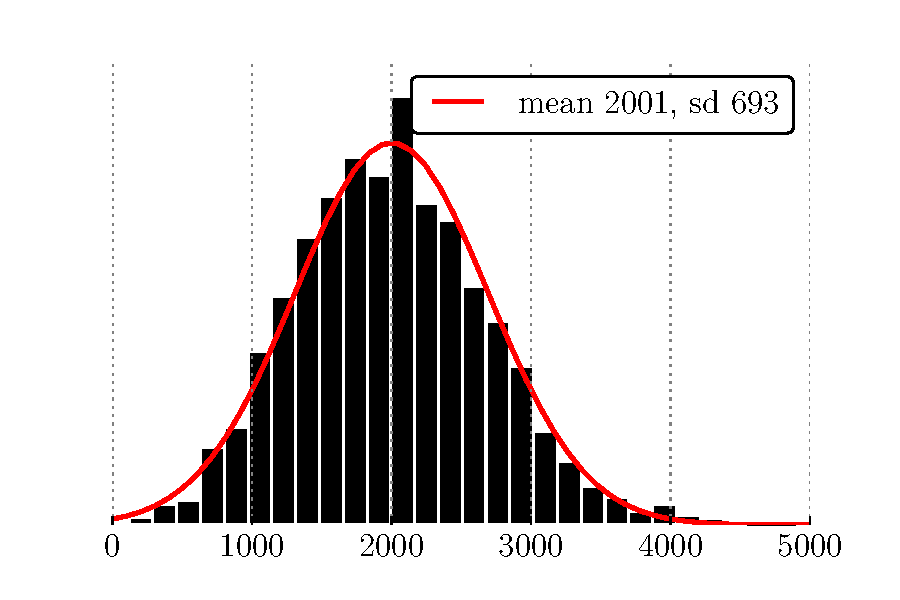
\includegraphics[width=.66\linewidth]{../ccnn/figures/roi_hist.pdf}
\caption{
Distribution of number of regions per image.
}\label{fig:roi_hist}
\end{figure}

\begin{figure}
\centering
\includegraphics[width=.66\linewidth]{../../figures/gradient_backprop.pdf}
\caption[Explanation of the gradient back-propagation quick feature.]{
As a quick feature, we back-propagate the gradient from the top classification layer all the way to the input pixels.
This induces a kind of saliency map on the image, which is useful signal for selecting image sub-regions to classify with the CNN.
}\label{fig:gradient_examples}
\end{figure}

\subsection{Cascade CNN}\label{sec:ccnn}

\PM{Motivation}
Despite the intentions of the region-proposal mechanism \parencite{Uijlings-IJCV-2013}, most ROIs that are scored in R-CNN do not contain any object of interest.
As in the classic cascade of \cite{Viola-IJCV-2004}, it would be useful to quickly reject these regions, without expending the full amount of computation on them.
The problem is that the deep neural network architecture is trained to always run all the way through.
We need to introduce a new primitive to enable early termination.

\PM{Method}
The Cascade CNN, shown in \autoref{fig:ccnn}, augments the CNN network with an ``Early Reject'' option: after some layers, the network decides whether to keep processing the input with the next layer.
Each reject layer is implemented as a fully-connected layer following a linear rectification, trained with dropout using logistic loss on foreground/background labels.
We first train an AlexNet-architecture network \parencite{Krizhevsky-NIPS-2012} on the ImageNet classification dataset.
This network is augmented with the Reject layers, its loss replaced with a multi-label cross-entropy loss, and fine-tuning on the PASCAL VOC training set is performed until loss stop decreasing (roughly 50000 iterations).
In training, all instances pass through all Reject layers.
After training, we set the reject thresholds to maintain at last 80\% recall at each stage, using a large sample of regions from images in the validation set containing positive and negative examples in equal proportion.

\PM{Implementation}
In the efficient implementation of CNNs we use (Caffe), there is a simple loop over each batch element in both CPU and GPU convolution code.
We modify this loop to simply not perform convolution on those elements that were rejected earlier in the cascade.
\footnote{While memory remains occupied in this scheme, we do not consider this a problem.}
Since most of the time is spent in the convolutional layers, we introduce a reject option after \texttt{pool1}, \texttt{pool2}, and \texttt{conv3}.
The last classification layer still outputs the full multi-class scores for the surviving regions.

\PM{Timing}
To estimate the saving on time by using the rejectors we timed the time spend to process 1000 regions (10 batches or 100) and the time expended in each of the first 3 layers:
\begin{itemize}
\item 1700 ms to process all the layers
\item 270 ms (15\%) in layer 1 (This includes \texttt{conv1}, \texttt{relu1}, \texttt{pool1}, \texttt{norm1})
\item 360 ms (20\%) in layer 2 (This includes \texttt{conv2}, \texttt{relu2}, \texttt{pool2}, \texttt{norm2})
\item 285 ms (15\%) in layer 3 (This includes \texttt{conv3}, \texttt{relu3})
\end{itemize}
Therefore the expected ``lifetimes'' of regions rejected after layer 1, layer 2, and layer 3 are  0.15, 0.35, and 0.5 of the total time taken per region.

\input{../ccnn/ccnn_fig}


%!TEX root=../paper/paper.tex
\section{Evaluation}\label{sec:ccnn_evaluation}

\PM{Dataset}
We evaluate on the standard object detection benchmark: the PASCAL VOC \cite{pascal-voc-2010}.
In all cases, the CNN region classifiers are trained on the PASCAL VOC 2007 trainval set.
The parameters of our methods are set by training or cross-validation on the VOC 2007 val set.
We evaluate on the VOC 2007 test set.
The result plots and details are shown in \autoref{fig:voc2007_results} and \autoref{tab:ccnn_results}.

\PM{Implementation}
The scoring function for the quick-to-compute features is trained by a logistic regression classifier onto the max PASCAL overlap with any ground truth window on the validation dataset.
The classifier is optimized by stochastic gradient descent, and its regularization parameter is cross-validated.
The R-CNN software was used as available in June 2014.
\footnote{\url{https://github.com/rbgirshick/rcnn}}
That software relies on Selective Search \cite{Uijlings-IJCV-2013} region proposals.
Different images are proposed different numbers of regions.
\autoref{fig:roi_hist} shows the distribution of number of regions on the validation set, with the parameters of the R-CNN.
An additional parameter is the size of each batch of regions that goes through the CNN.
We set batch size to 100 regions, and observe that it takes on average 500 ms to process them with the CNN.
In all experiments, we use Ubuntu 12.04, Intel i5 3.2GHz CPU, and NVIDIA Tesla K40 GPU.

\input{../ccnn/voc2007_fig}

\input{../ccnn/voc2007_table}

The experimental settings are
\begin{description}
  \item[Original] \hfill \\
  The original order of the Selective Search regions of interest.
  This order is influenced by the hierarchical segmentation of their method, and so has sequences of highly overlapping regions.

  \item[Random] \hfill \\
  A completely blind permutation of the original order.

  \item[Region Selection] \hfill \\
  The region statistics feature is always used.
  Additionally, we consider the Pixel Gradient feature, with \emph{setup time} of the gradient forward-back propagation of 20 ms.

  \item[Cascade CNN] \hfill \\
  The Cascade CNN model, as described in \autoref{sec:ccnn}.
  The first experiment (C-CNN) takes batches of regions in a random order.
  The next two experiments also make use of the Region Selection methodology with the quick-to-compute feature.
\end{description}

\PM{Analysis}
Since the time to process a full batch with a non-Cascade CNN is 500 ms, there are no results for non-cascaded baselines at 300 ms.
At this time, the Cascade CNN without any region ordering is best.
A reason for why C-CNN with Region Selection is not as good at this point is that the region selection presents better region candidates, with fewer rejection opportunities, and thus has less coverage of the image.
At 600 ms, C-CNN method have had more than one batch go through, and the Region Selection is giving it a lead over the simple C-CNN.
Both method are better than the baseline non-cascaded methods for this entire duration.


%!TEX root=../paper/paper.tex
\chapter{Recognizing Image Style}\label{sec:style_chapter}

\begin{figure}[t]
\small{
\centering
\begin{subfigure}[t]{0.48\linewidth}
    \begin{tabular}{cc}
        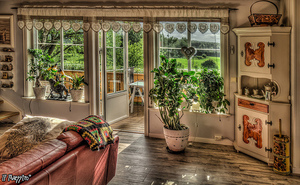
\includegraphics[width=.43\linewidth]{../style/figures/flickrDatasetExamples/used/resized/hdr.jpg} &
    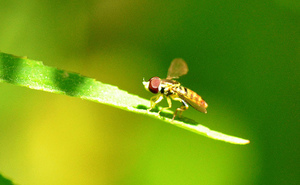
\includegraphics[width=.43\linewidth]{../style/figures/flickrDatasetExamples/used/resized/macro.jpg} \\
    HDR & Macro \\
        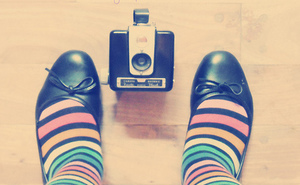
\includegraphics[width=.43\linewidth]{../style/figures/flickrDatasetExamples/used/resized/vintage.jpg} &
    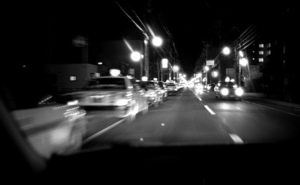
\includegraphics[width=.43\linewidth]{../style/figures/flickrDatasetExamples/used/resized/noir.jpg} \\
    Vintage & Noir \\
        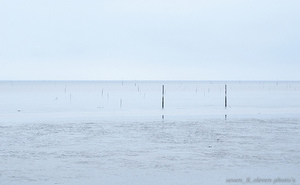
\includegraphics[width=.43\linewidth]{../style/figures/flickrDatasetExamples/used/resized/minimal.jpg} &
    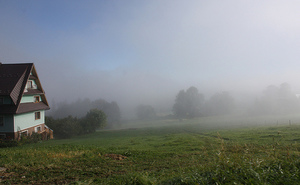
\includegraphics[width=.43\linewidth]{../style/figures/flickrDatasetExamples/used/resized/hazy.jpg} \\
    Minimal & Hazy \\
        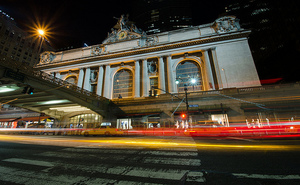
\includegraphics[width=.43\linewidth]{../style/figures/flickrDatasetExamples/used/resized/long_exposure.jpg} &
    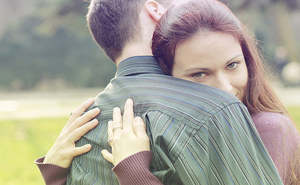
\includegraphics[width=.43\linewidth]{../style/figures/flickrDatasetExamples/used/resized/romantic.jpg} \\
    Long Exposure & Romantic \\
    \end{tabular}
    \caption{
        Flickr Style: 80K images covering 20 styles.
    }\label{fig:flickr_style_examples}
\end{subfigure}\hspace{2em}\begin{subfigure}[t]{0.48\linewidth}
    \begin{tabular}{cc}
        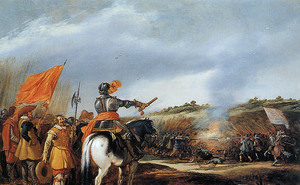
\includegraphics[width=.43\linewidth]{../style/figures/wikipaintingsDatasetExamples/used/resized/baroque-0.jpg} &
    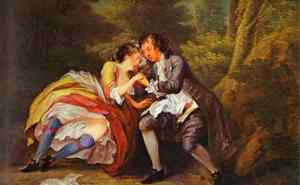
\includegraphics[width=.43\linewidth]{../style/figures/wikipaintingsDatasetExamples/used/resized/roccoco-0.jpg} \\
    Baroque & Roccoco \\
        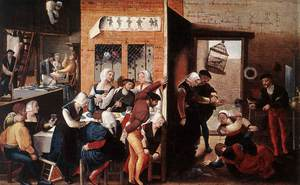
\includegraphics[width=.43\linewidth]{../style/figures/wikipaintingsDatasetExamples/used/resized/northern_renaissance-0.jpg} &
        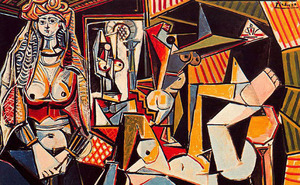
\includegraphics[width=.43\linewidth]{../style/figures/wikipaintingsDatasetExamples/used/resized/cubism-0.jpg} \\
    Northern Renaissance & Cubism \\
        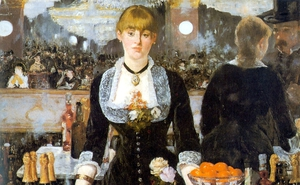
\includegraphics[width=.43\linewidth]{../style/figures/wikipaintingsDatasetExamples/used/resized/impressionism-0.jpg} &
        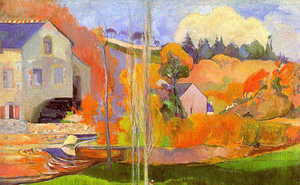
\includegraphics[width=.43\linewidth]{../style/figures/wikipaintingsDatasetExamples/used/resized/post_impressionism-0.jpg} \\
    Impressionism & Post-Impressionism \\
        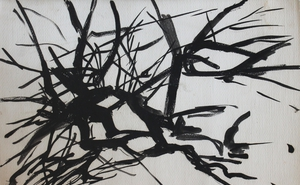
\includegraphics[width=.43\linewidth]{../style/figures/wikipaintingsDatasetExamples/used/resized/abs_expressionism-0.jpg} &
    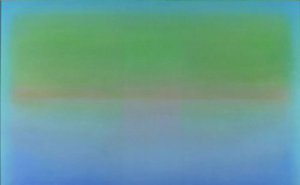
\includegraphics[width=.43\linewidth]{../style/figures/wikipaintingsDatasetExamples/used/resized/color_field-0.jpg} \\
    Abs. Expressionism & Color Field Painting \\
    \end{tabular}
    \caption{
        Wikipaintings: 85K images for 25 genres.
    }\label{fig:wikipaintings_style_examples}
\end{subfigure}
}
\caption{
    Typical images in different style categories of our datasets.
}\label{fig:style_examples}
\end{figure}

\PM{Motivation}
Deliberately-created images convey meaning, and \textit{visual style} is often a significant component of image meaning.
For example, a political candidate portrait made in the lush colors of a Renoir painting tells a different story than if it were in the harsh, dark tones of a horror movie.
Distinct visual styles are apparent in art, cinematography, advertising, and have become extremely popular in amateur photography, with apps like Instagram leading the way.
While understanding style is crucial to image understanding, very little research in computer vision has explored visual style.

\PM{Definition}
We define several different \textit{types} of image style, and gather a new, large-scale dataset of photographs annotated with style labels.
This dataset embodies several different aspects of visual style, including photographic techniques  (``Macro,'' ``HDR''), composition styles (``Minimal,'' ``Geometric''), moods (``Serene,'' ``Melancholy''), genres (``Vintage,'' ``Romantic,'' ``Horror''), and types of scenes (``Hazy,'' ``Sunny'').
These styles are not mutually exclusive, and represent different attributes of style.
We also gather a large dataset of visual art (mostly paintings) annotated with art historical style labels, ranging from Renaissance to modern art.
\autoref{fig:style_examples} shows some samples.
Analyzing style of non-photorealistic media is interesting as much of our present understanding of visual style arises out of thousands of years of developments in fine art, marked by distinct historical styles.

\section{Method}\label{sec:style_method}

\PM{Approach}
We test existing classification algorithms on these styles, evaluating several state-of-the-art image features.
Most previous work in aesthetic style analysis has  used hand-tuned features, such as color histograms.
We find that deep convolutional neural network (CNN) features perform best for the task.
This is surprising for several reasons: these features were trained on object class categories (ImageNet), and many styles appear to be primarily about color choices, yet the CNN features handily beat color histogram features.
This leads to one conclusion of our work: mid-level features derived from object datasets are generic for style recognition, and superior to hand-tuned features.
We compare our predictors to human observers, using Amazon Mechanical Turk experiments, and find that our classifiers predict Group membership at essentially the same level of accuracy as Turkers.
We also test on the AVA aesthetic prediction task \parencite{Murray-CVPR-2012}, and show that using the ``deep'' object recognition features improves over the state-of-the-art results.

\PM{Applications and code}
First, we demonstrate an example of using our method to search for images by style.
This could be useful for applications such as product search, storytelling, and creating slide presentations.
In the same vein, visual similarity search results could be filtered by visual style, making possible queries such as ``similar to this image, but more Film Noir.''
Second, style tags may provide valuable mid-level features for other image understanding tasks.
For example, there has increasing recent effort in understanding image meaning, aesthetics, interestingness, popularity, and emotion (for example, \parencite{Gygli-ICCV-2013,Isola-CVPR-2011,joo2014,khosla2014}), and style is an important part of meaning.
Finally, learned predictors could be a useful component in modifying the style of an image.
All data, trained predictors, and code (including results viewing interface) are available at \url{http://sergeykarayev.com/recognizing-image-style/}.

\subsection{Data Sources}

\PM{Motivation}
Building an effective model of photographic style requires annotated training data.  To our knowledge, there is only one existing dataset annotated with visual style, and only a narrow range of photographic styles is represented~\parencite{Murray-CVPR-2012}.
We would like to study a broader range of styles, including different \textit{types} of styles ranging from genres, compositional styles, and moods.
Morever, large datasets are desirable in order to obtain effective results, and so we would like to obtain data from online communities, such as Flickr.

\subsubsection{Flickr Style}

\PM{Source}
Although Flickr users often provide free-form tags for their uploaded images, the tags tend to be quite unreliable.
Instead, we turn to Flickr groups, which are community-curated collections of visual concepts.
For example, the Flickr Group ``Geometry Beauty'' is described, in part, as ``Circles, triangles, rectangles, symmetric objects, repeated patterns'', and contains over 167K images at time of writing; the ``Film Noir Mood'' group is described as ``Not just  black and white photography, but a dark, gritty, moody feel...'' and comprises over 7K images.

At the outset, we decided on a set of 20 visual styles, further categorized into types:
\begin{itemize} \itemsep0.5pt
\item \textbf{Optical techniques:} Macro, Bokeh, Depth-of-Field, Long Exposure, HDR
\item \textbf{Atmosphere:} Hazy, Sunny
\item \textbf{Mood:} Serene, Melancholy, Ethereal
\item \textbf{Composition styles:} Minimal, Geometric, Detailed, Texture
\item \textbf{Color:} Pastel, Bright
\item \textbf{Genre:} Noir, Vintage, Romantic, Horror
\end{itemize}

For each of these stylistic concepts, we found at least one dedicated Flickr Group with clearly defined membership rules.
From these groups, we collected 4,000 positive examples for each label, for a total of 80,000 images.
Example images are shown in \autoref{fig:flickr_style_examples}.

\PM{Dealing with Noise}
The derived labels are considered clean in the positive examples, but may be noisy in the negative examples, in the same way as the ImageNet dataset \parencite{Deng-CVPR-2009}.
That is, a picture labeled as \emph{Sunny} is indeed \emph{Sunny}, but it may also be \emph{Romantic}, for which it is not labeled.
We consider this an unfortunate but acceptable reality of working with a large-scale dataset.
Following ImageNet, we still treat the absence of a label as indication that the image is a negative example for that label.
Mechanical Turk experiments described in \autoref{sec:mech_turk_evaluation} serve to allay our concerns.

\subsubsection{Wikipaintings}

\PM{Source}
We also provide a new dataset for classifying painting style.
To our knowledge, no previous large-scale dataset exists for this task -- although very recently a large dataset of artwork did appear for other tasks \parencite{Mensink2014}.
We collect a dataset of 100,000 high-art images -- mostly paintings -- labeled with artist, style, genre, date, and free-form tag information by a community of experts on the \texttt{Wikipaintings.org} website.
Our dataset presents significant stylistic diversity, primarily spanning Renaissance styles to modern art movements.% (\autoref{fig:wikipaintings_data} provides further breakdowns).
We select 25 styles with more than 1,000 examples, for a total of 85,000 images.
Example images are shown in~\autoref{fig:wikipaintings_style_examples}.

\subsection{Learning algorithm}

\PM{Multi-Class Logistic Regression via SGD}
We learn to classify novel images according to their style, using the labels assembled in the previous section.
Because the datasets we deal with are quite large and some of the features are high-dimensional, we consider only linear classifiers, relying on sophisticated features to provide robustiness.
We use an open-source implementation of Stochastic Gradient Descent with adaptive subgradient \parencite{Agarwal-JMLR-2012}.
The learning process optimizes the function \[
\underset{w}{\text{min }} \lambda_1 \|w\|_1 + \frac{\lambda_2}{2} \Vert w \Vert_2^2 + \sum_i \ell(x_i, y_i, w)
\]
We set the $L_1$ and $L_2$ regularization parameters and the form of the loss function by validation on a held-out set.
For the loss $\ell(x, y, w)$, we consider the hinge ($\max(0, 1 - y \cdot w^T x)$) and logistic ($\log(1 + \exp(-y \cdot w^T x))$) functions.
We set the initial learning rate to $0.5$, and use adaptive subgradient optimization~\parencite{duchi2011adaptive}.
Our setup is of multi-class classification; we use the One vs. All reduction to binary classifiers.

\subsection{Image Features}

\PM{Motivation}
In order to classify styles, we must choose appropriate image features.  We hypothesize that image style may be related to many different features, including low-level statistics \parencite{Lyu-PNAS-2004}, color choices, composition, and content.  Hence, we test features that embody these different elements, including features from the object recognition literature.
We evaluate single-feature performance, as well as second-stage fusion of multiple features.

\paragraph{L*a*b color histogram.}
Many of the Flickr styles exhibit strong dependence on color. For example, \emph{Noir} images are nearly all black-and-white, while most \emph{Horror} images are very dark, and \emph{Vintage} images use old photographic colors. We use a standard color histogram feature, computed on the whole image.
The 784-dimensional joint histogram in CIELAB color space has 4, 14, and 14 bins in the L*, a*, and b* channels, following Palermo et al.~\parencite{Palermo-ECCV-2012}, who showed this to be the best performing single feature for determining the date of historical color images.

\paragraph{GIST.}
The classic gist descriptor \parencite{Oliva-IJCV-2001} is known to perform well for scene classification and retrieval of images visually similar at a low-resolution scale, and thus can represent image composition to some extent.
We use the INRIA LEAR implementation, resizing images to 256 by 256 pixels and extracting a 960-dimensional color GIST feature.

\paragraph{Graph-based visual saliency.}
We also model composition with a visual attention feature \parencite{Harel-NIPS-2006}.
The feature is fast to compute and has been shown to predict human fixations in natural images basically as well as an individual human (humans are far better in aggregate, however).
The 1024-dimensional feature is computed from images resized to 256 by 256 pixels.

\paragraph{Meta-class binary features.}
Image content can be predictive of individual styles, e.g., \emph{Macro} images include many images of insects and flowers. The \texttt{mc-bit} feature~\parencite{Bergamo-CVPR-2012} is a 15,000-dimensional bit vector feature learned as a non-linear combination of classifiers trained using existing features (e.g., SIFT, GIST, Self-Similarity) on thousands of random ImageNet synsets, including internal ILSVRC2010 nodes.
In essence, MC-bit is a hand-crafted ``deep'' architecture, stacking classifiers and pooling operations on top of lower-level features.

\paragraph{Deep convolutional net.}
Current state-of-the-art results on ImageNet, the largest image classification challenge, have come from a deep convolutional network trained in a fully-supervised manner \parencite{krizhevsky2012imagenet}.
We use the Caffe \parencite{Jia13caffe} open-source implementation of the ImageNet-winning eght-layer convolutional network, trained on over a million images annotated with 1,000 ImageNet classes.
We investigate using features from two different levels of the network, referred to as DeCAF$_5$ and DeCAF$_6$ (following \parencite{Donahue2013}).
The features are 8,000- and 4,000-dimensional and are computed from images center-cropped and resized to 256 by 256 pixels.

\paragraph{Content classifiers.}
Following Dhar et al.~\parencite{Dhar-CVPR-2011}, who use high-level classifiers as features for their aesthetic rating prediction task, we evaluate using object classifier confidences as features.
Specifically, we train classifiers for all 20 classes of the PASCAL VOC \parencite{pascal-voc-2010} using the DeCAF$_6$ feature.
The resulting classifiers are quite reliable, obtaining $0.7$ mean AP on the VOC 2012.
We aggregate the data to train four classifiers for ``animals'', ``vehicles'', ``indoor objects'' and ``people''.

\paragraph{Fusion.}
These aggregate classes are presumed to discriminate between vastly different types of images -- types for which different style signals may apply.
For example, a \emph{Romantic} scene with people may be largely about the composition of the scene, whereas, \emph{Romantic} scenes with vehicles may be largely described by color.
To enable our classifiers to learn content-dependent style, we can take the outer product of a feature channel with the four aggregate content classifiers.

\section{Evaluation}\label{sec:style_evaluation}

\begin{table}
\caption[Mean APs on AVA Style, Flickr Style, and Wikipaintings for single-channel features and their second-stage combinations.]{
    Mean APs on three datasets for the considered single-channel features and their second-stage combination.
    As some features were clearly worse than others on the AVA Style dataset, only the better features were evaluated on larger datasets.
}
\label{tab:mean_aps}
\centering
\vspace{1em}
\footnotesize{
\begin{tabular}{lrrrrrrrrr}
\toprule
{}                & Fusion x Content & DeCAF$_6$ & MC-bit & L*a*b* Hist & GIST  & Saliency & random \\
\midrule
AVA Style         & \textbf{0.581}   & 0.579     & 0.539  & 0.288       & 0.220 & 0.152    & 0.132 \\
Flickr            & \textbf{0.368}   & 0.336     & 0.328  & -           & -     & -        & 0.052 \\
Wikipaintings     & \textbf{0.473}   & 0.356     & 0.441  & -           & -     & -        & 0.043 \\
\bottomrule
\end{tabular}
}
\end{table}

\subsection{Experiment: Flickr Style}

\PM{Setup}
We learn and predict style labels on the 80,000 images labeled with 20 different visual styles of our new Flickr Style dataset, using 20\% of the data for testing, and another 20\% for parameter-tuning validation.
There are several performance metrics we consider.
Average Precision evaluation (as reported in \autoref{tab:mean_aps} and in \autoref{tab:flickr_ap_table}) is computed on a random class-balanced subset of the test data (each class has equal prevalence).
%We compute confusion matrices (\autoref{fig:flickr_conf}, \autoref{fig:wp_conf}, \autoref{fig:ava_style_conf}) on the same data.
We compute confusion matrices (\autoref{fig:flickr_conf}, \autoref{fig:wp_conf}) on the same data.
Per-class accuracies are computed on subsets of the data balanced by the binary label, such that chance performance is 50\%.
We follow these decisions in all following experiments.

\PM{Single features}
The best single-channel feature is DeCAF$_6$ with 0.336 mean AP; feature fusion obtains 0.368 mean AP.
Per-class APs range from 0.17 [\emph{Depth of Field}] to  0.62 [\emph{Macro}].
Per-class accuracies range from 68\% [\emph{Romantic}, \emph{Depth of Field}] to 85\% [\emph{Sunny}, \emph{Noir}, \emph{Macro}].
The average per-class accuracy is 78\%.
We show the most confident style classifications on the test set of Flickr Style in \autoref{fig:flickr_on_flickr1} through \autoref{fig:flickr_on_flickr3}.

\PM{Analysis}
Upon inspection of the confusion matrices, we saw points of understandable confusion: \emph{Depth of Field} vs. \emph{Macro}, \emph{Romantic} vs. \emph{Pastel}, \emph{Vintage} vs. \emph{Melancholy}.
There are also surprising sources of mistakes: \emph{Macro} vs. \emph{Bright/Energetic}, for example.
To explain this particular confusion, we observed that lots of \emph{Macro} photos contain bright flowers, insects, or birds, often against vibrant greenery.
Here, at least, the content of the image dominates its style label.
To explore further content-style correlations, we plot the outputs of PASCAL object class classifiers (one of our features) on the Flickr dataset in~\autoref{fig:content_correlation}.
We can observe that some styles have strong correlations to content (e.g., \emph{Hazy} occurs with \emph{vehicle}, \emph{HDR} doesn't occur with \emph{cat}).

\PM{Fusion}
We hypothesize that style is content-dependent: a \emph{Romantic} portrait may have different low-level properties than a \emph{Romantic} sunset.
We form a new feature as an outer product of our content classifier features with the second-stage late fusion features (``Fusion $\times$ Content'' in all results figures).
These features gave the best results, thus supporting the hypothesis.

\begin{figure}[h]
\centering
    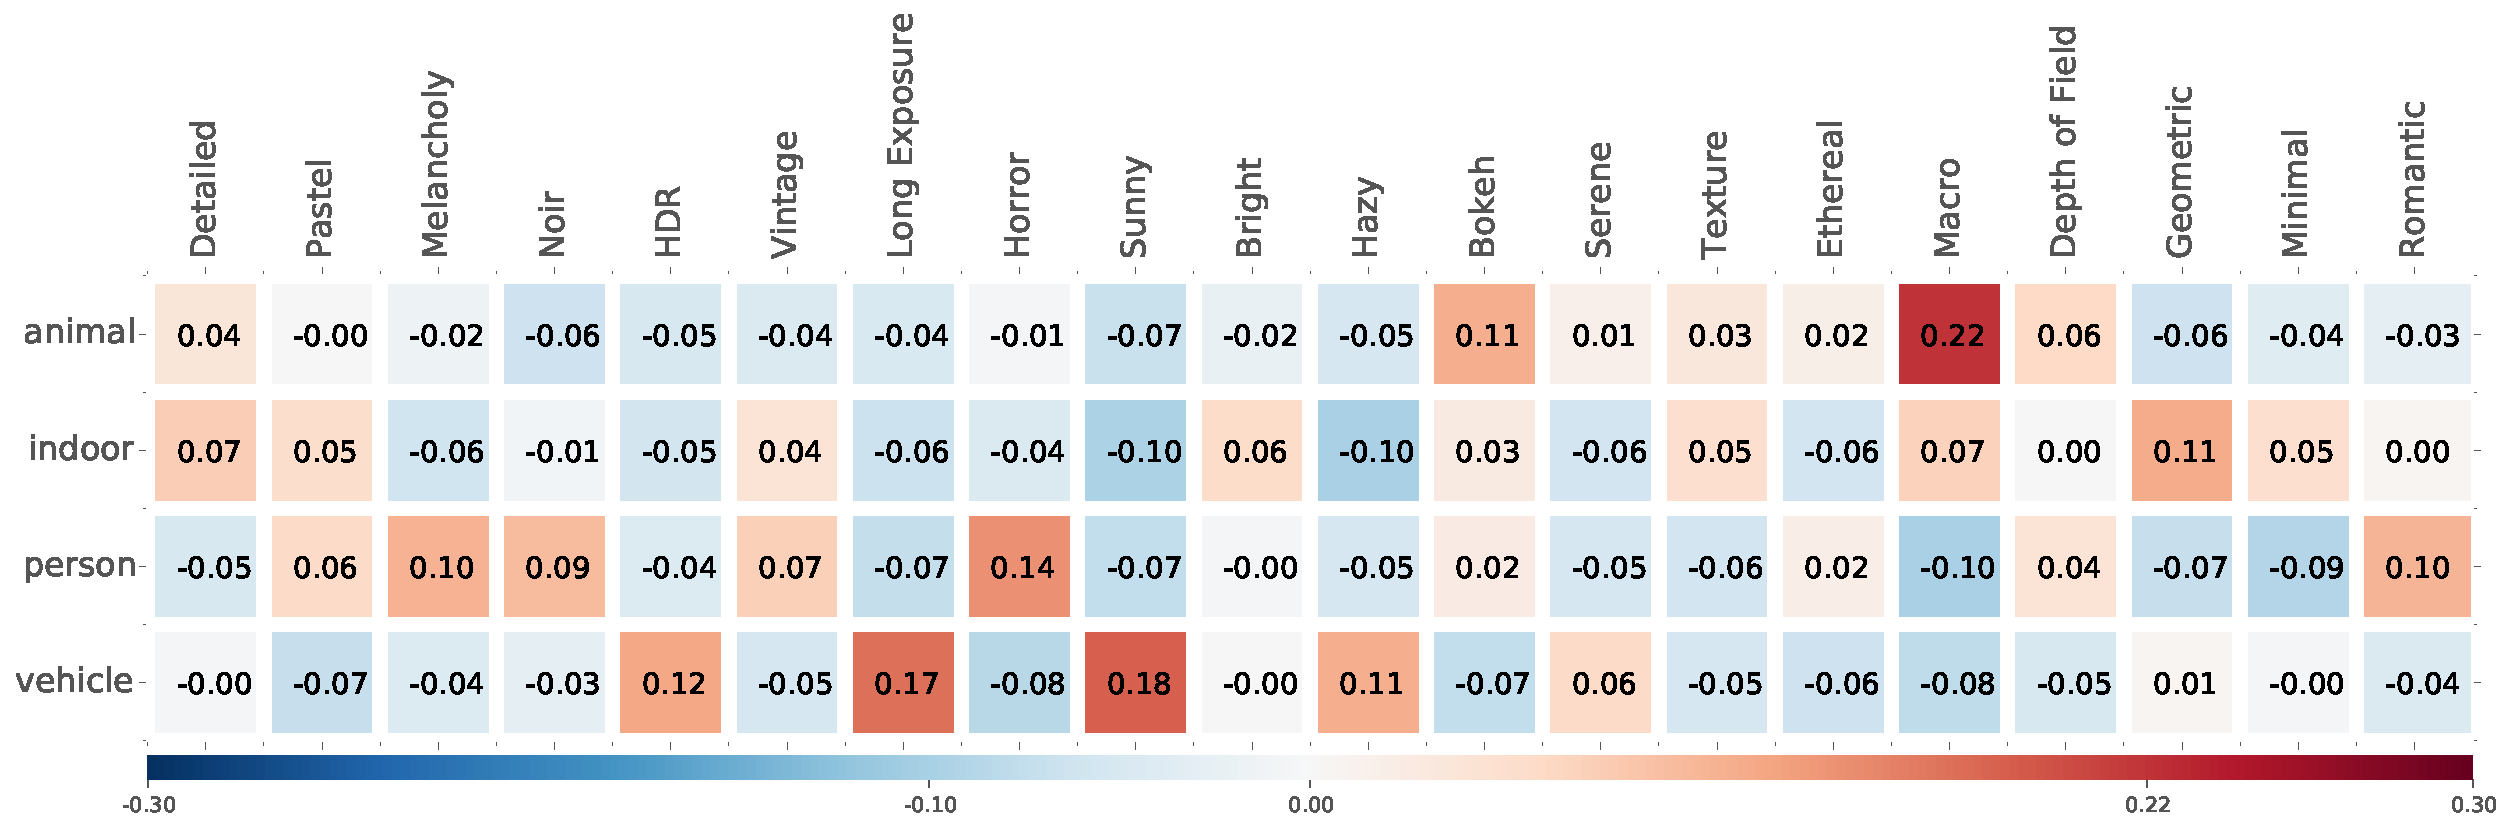
\includegraphics[width=\linewidth]{../style/figures/content_correlation2/pascal_on_flickr.pdf}
    \caption[Correlation of PASCAL content classifier predictions with ground truth Flickr Style labels.]{
        Correlation of PASCAL content classifier predictions (rows) against ground truth Flickr Style labels (columns).
        We see, for instance, that the Macro style is highly correlated with presence of animals, and that Long Exposure and Sunny style photographs often feature vehicles.
    }\label{fig:content_correlation}
\end{figure}

\subsubsection{Mechanical Turk Evaluation}\label{sec:mech_turk_evaluation}

\PM{Setup}
In order to provide a human baseline for evaluation, we performed a Mechanical Turk study.
For each style, Turkers were shown positive and negative examples for each Flickr Group, and then they evaluated whether each image in the test set was part of the given style.
We treat the Flickr group memberships as ground truth as before, and then evaluate Turkers' ability to accurately determine group membership.
Measures were taken to remove spam workers, as described below.
For efficiency, one quarter of the test set was used, and two redundant styles (Bokeh and Detailed) were removed.
Each test image was evaluated by 3 Turkers, and the majority vote taken as the human result for this image.

\PM{Details}
Test images were grouped into 10 images per Human Interface Task (HIT). Each task asks the Turker to evaluate the style (e.g., ``Is this image VINTAGE?'') for each image.  For each style, we provided a short blurb describing the style in words, and provided 12-15 hand-chosen positive and negative examples for each Flickr Group.
To defend against spammers, each HIT included 2 sentinels: images which were very clearly positives and similar to the examples.  HITs were rejected when Turkers got both sentinels wrong.
Turkers were paid $0.10$ per HIT, and were allowed to perform multiple hits.  Manual inspection of the results indicate that the Turkers understood the task and were performing effectively.  A few Turkers sent unsolicited feedback indicating that they were really enjoying the HITs (``some of the photos are beautiful'') and wanted to perform them as effectively as possible.

\PM{Results}
Results are presented in \autoref{tab:flickr_vs_mturk} and \autoref{tab:flickr_vs_mturk2}.
In total, Turkers achieved 75\% mean accuracy (ranging from 61\% [\emph{Romantic}] to 92\% [\emph{Macro}]) across styles, in comparison to 78\% mean accuracy (ranging from 68\% [\emph{Depth of Field}] to 87\% [\emph{Macro}]) of our best method.
Our algorithm did significantly worse than Turkers on \emph{Macro} and \emph{Horror}, and significantly better on \emph{Vintage}, \emph{Romantic}, \emph{Pastel}, \emph{Detailed}, \emph{HDR}, and \emph{Long Exposure} styles.
We additionally used the Turker opinion as ground truth for our method's predictions.
In switching from the default Flickr to the MTurk ground truth, our method's accuracy hardly changed from 78\% to 77\%.
However, we saw that the accuracy of our \emph{Vintage}, \emph{Detailed}, \emph{Long Exposure}, \emph{Minimal}, \emph{HDR}, and \emph{Sunny} style classifiers significantly decreased, indicating machine-human disagreement on those styles.

\PM{Analysis}
Some of this variance may be due to subtle difference from the Turk tasks that we provided, as compared to the definitions of the Flickr groups, but may also due to the Flickr groups' incorporating images that do not quite fit the common definition of the given style.
For example, there may be a mismatch between different notions of \emph{Romantic} and \emph{vintage}, and how inclusively these terms are defined.
Regardless, the high agreement seen in study validates our choice of data source.

\subsection{Experiment: Wikipaintings}

\PM{Setup and Results}
With the same setup and features as in the Flickr experiments, we evaluate 85,000 images labeled with 25 different art styles.
Detailed results are provided in \autoref{tab:wikipaintings_ap_table} and \autoref{tab:wp_accuracies}.
The best single-channel feature is MC-bit with 0.441 mean AP; feature fusion obtains 0.473 mean AP.
Per-class accuracies range from 72\% [\emph{Symbolism}, \emph{Expressionism}, \emph{Art Nouveau}] to 94\% [\emph{Ukiyo-e}, \emph{Minimalism}, \emph{Color Field Painting}].
We did not perform a Mechanical Turk analysis of this dataset, as the Wikipainting community-of-experts labels were deemed inherently less noisy than Flickr Groups.

\subsection{Experiment: AVA Style}

\PM{Setup and Results}
AVA \parencite{Murray-CVPR-2012} is a dataset of 250K images from \texttt{dpchallenge.net}.
We evaluate classification of aesthetic rating and of 14 different photographic style labels on the 14,000 images of the AVA dataset that have such labels.
For the style labels, the publishers of the dataset provide a train/test split, where training images have only one label, but test images may have more than one label \parencite{Murray-CVPR-2012}.
Our results are presented in \autoref{tab:ava_style_ap_table}.
For style classification, the best single feature is the DeCAF$_6$ convolution network feature, obtaining 0.579 mean AP.
Feature fusion improves the result to 0.581 mean AP; both results beat the previous state-of-the-art of 0.538 mean AP \parencite{Murray-CVPR-2012}.
Our results beat 0.54 mAP using both the AVA-provided class-imbalanced test split, and the class-balanced subsample that we consider to be more correct evaluation, and for which we provide numbers.

\PM{Low-level features}
In all metrics, the DeCAF and MC-bit features significantly outperformed more low-level features on this dataset.
For this reason, we did not evaluate the low-level features on the larger Flickr and Wikipaintings datasets (the AVA experiment was chronologically first).

\subsection{Application: Style-Based Image Search}

\PM{Cross-dataset style}
Style classifiers learned on our datasets can be used toward novel goals.
For example, sources of stock photography or design inspiration may be better navigated with a vocabulary of style.
Currently, companies expend labor to manually annotate stock photography with such labels.
With our approach, any image collection can be searchable and rankable by style.
To demonstrate, we apply our Flickr-learned style classifiers to a new dataset of 80K images gathered on Pinterest (also available with our code release); some results are shown in \autoref{fig:flickr_on_pinterest}.
Interestingly, styles learned from photographs can be used to order paintings, and styles learned from paintings can be used to order photographs, as illustrated in \autoref{fig:photo_painting}.

\begin{figure*}[ht]
\centering
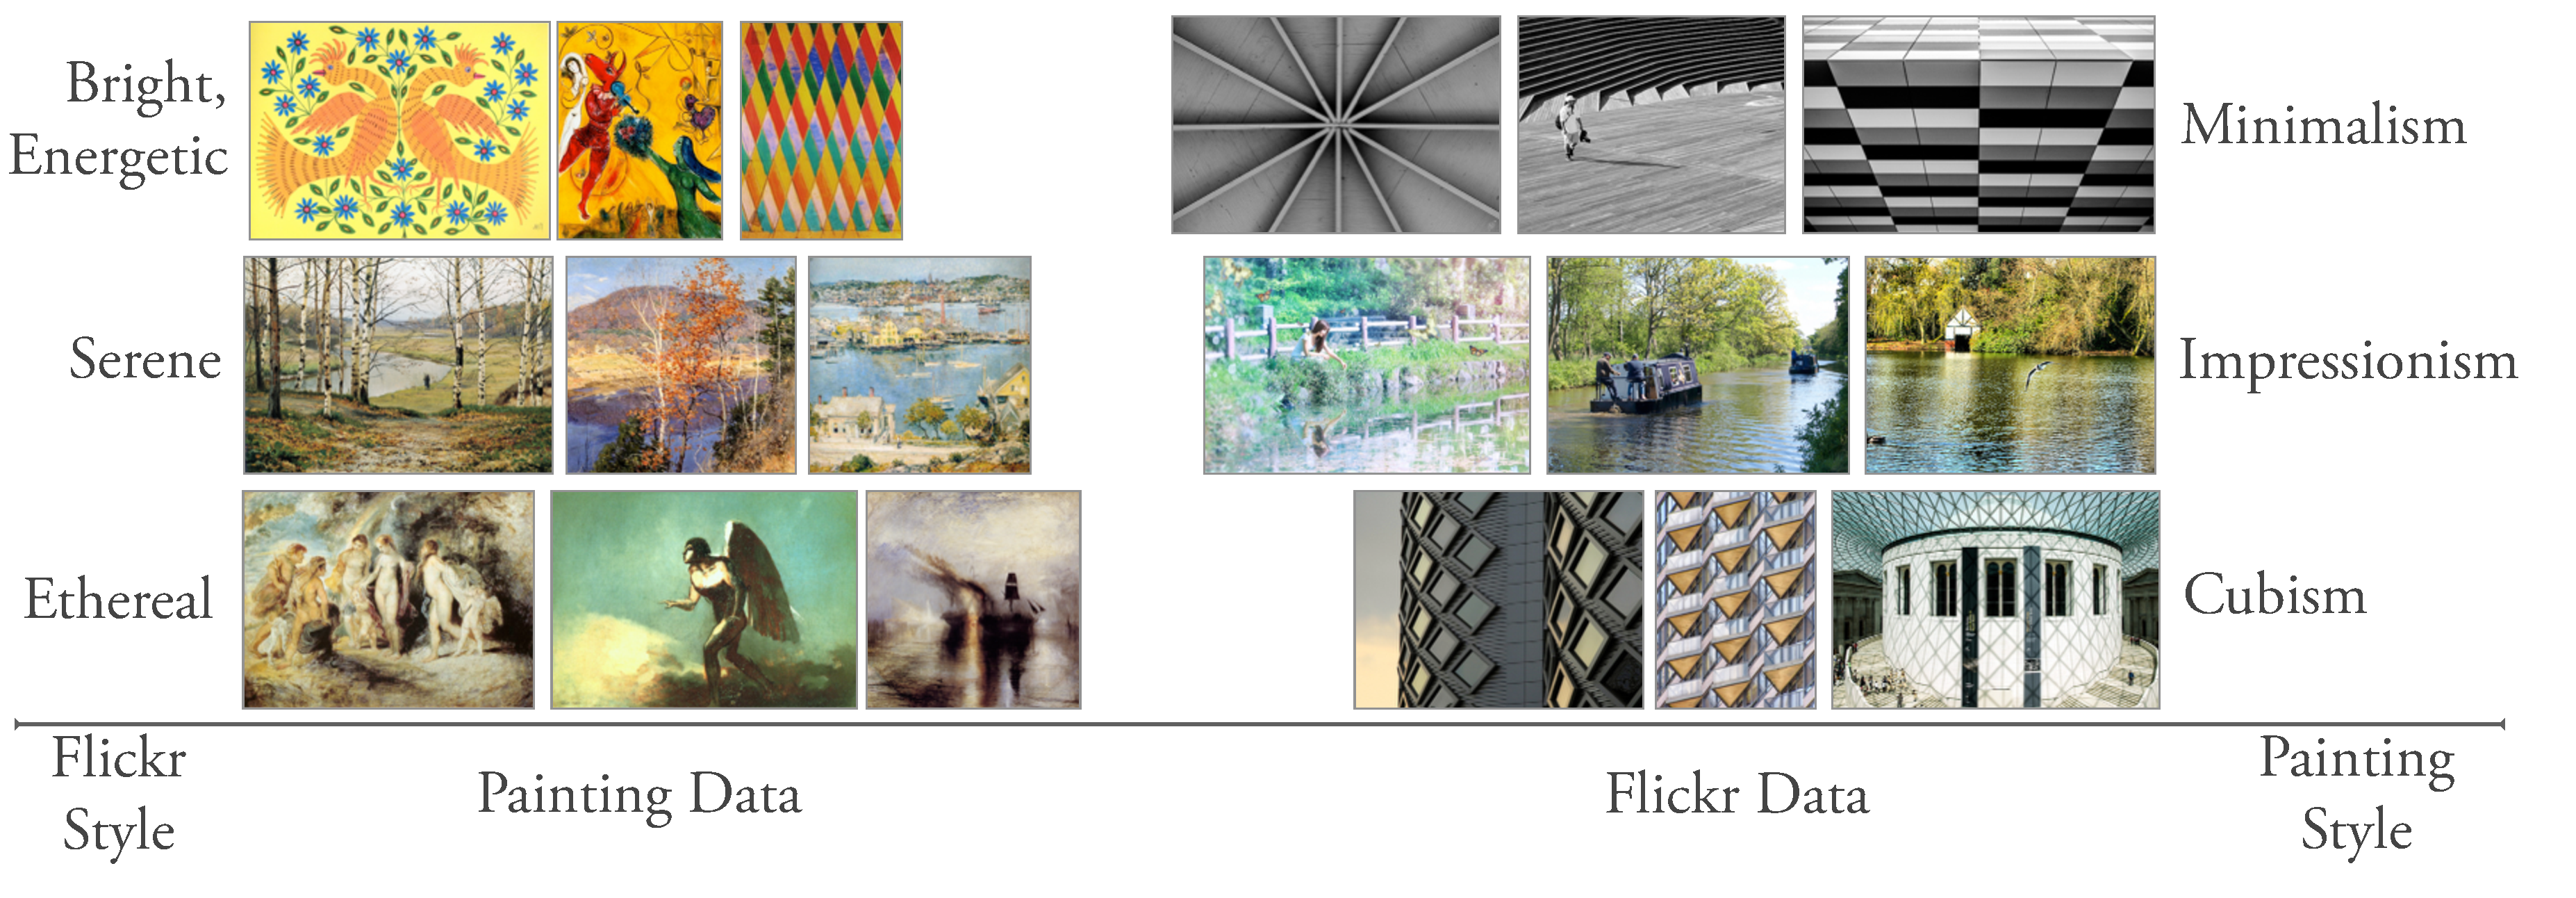
\includegraphics[width=\linewidth]{../style/figures/style_by_style.pdf}
\caption[Cross-dataset understanding of style demonstrated by applying Wikipaintings-learned classifiers to phoitographs, and Flickr-learned classifiers to paintings.]{
    Cross-dataset style.
    On the left are shown top scorers from the Wikipaintings set, for styles learned on the Flickr set.
    On the right, Flickr photographs are accordingly sorted by Painting style.
    (Figure best viewed in color.)
}
\label{fig:photo_painting}
\end{figure*}

\newcommand{\dgap}{.65in}
\begin{figure}
\begin{subfigure}[t]{0.48\linewidth}
    \begin{tabular}{m{.05in}|m{\dgap} m{\dgap} m{\dgap}}
    \begin{turn}{90}\small{Bright}\end{turn} &
    \includegraphics[width=.8in]{../style/figures/flickr_on_pinterest/dress/pred_style_Bright/h/0.jpg} &
    \includegraphics[width=.8in]{../style/figures/flickr_on_pinterest/dress/pred_style_Bright/h/1.jpg} &
    \includegraphics[width=.8in]{../style/figures/flickr_on_pinterest/dress/pred_style_Bright/h/2.jpg} \\ \\
    \begin{turn}{90}\small{Pastel}\end{turn} &
    \includegraphics[width=.8in]{../style/figures/flickr_on_pinterest/dress/pred_style_Pastel/h/0.jpg} &
    \includegraphics[width=.8in]{../style/figures/flickr_on_pinterest/dress/pred_style_Pastel/h/1.jpg} &
    \includegraphics[width=.8in]{../style/figures/flickr_on_pinterest/dress/pred_style_Pastel/h/2.jpg} \\ \\
    \begin{turn}{90}\small{Ethereal}\end{turn} &
    \includegraphics[width=.8in]{../style/figures/flickr_on_pinterest/dress/pred_style_Ethereal/h/0.jpg} &
    \includegraphics[width=.8in]{../style/figures/flickr_on_pinterest/dress/pred_style_Ethereal/h/1.jpg} &
    \includegraphics[width=.8in]{../style/figures/flickr_on_pinterest/dress/pred_style_Ethereal/h/2.jpg} \\ \\
    \begin{turn}{90}\small{Noir}\end{turn} &
    \includegraphics[width=.8in]{../style/figures/flickr_on_pinterest/dress/pred_style_Noir/h/0.jpg} &
    \includegraphics[width=.8in]{../style/figures/flickr_on_pinterest/dress/pred_style_Noir/h/1.jpg} &
    \includegraphics[width=.8in]{../style/figures/flickr_on_pinterest/dress/pred_style_Noir/h/2.jpg} \\ \\
    \begin{turn}{90}\small{Vintage}\end{turn} &
    \includegraphics[width=.8in]{../style/figures/flickr_on_pinterest/flower/pred_style_Vintage/h/0.jpg} &
    \includegraphics[width=.8in]{../style/figures/flickr_on_pinterest/flower/pred_style_Vintage/h/2.jpg} &
    \includegraphics[width=.8in]{../style/figures/flickr_on_pinterest/flower/pred_style_Vintage/h/3.jpg} \\
    \end{tabular}
    \caption{Query: ``dress''.}
\end{subfigure}\hfill\begin{subfigure}[t]{0.48\linewidth}
    \begin{tabular}{m{.05in}|m{\dgap} m{\dgap} m{\dgap}}
    \begin{turn}{90}\small{DoF}\end{turn} &
    \includegraphics[width=.8in]{../style/figures/flickr_on_pinterest/flower/pred_style_Depth_of_Field/h/1.jpg} &
    \includegraphics[width=.8in]{../style/figures/flickr_on_pinterest/flower/pred_style_Depth_of_Field/h/3.jpg} &
    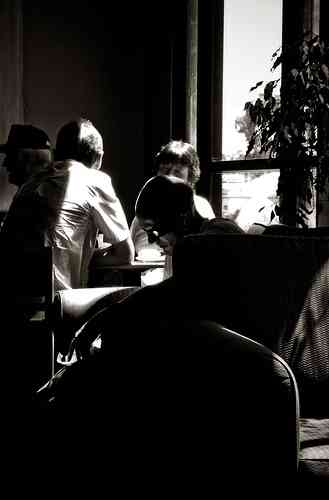
\includegraphics[width=.8in]{../style/figures/flickr_on_pinterest/flower/pred_style_Depth_of_Field/h/4.jpg} \\ \\
    \begin{turn}{90}\small{Romantic}\end{turn} &
    \includegraphics[width=.8in]{../style/figures/flickr_on_pinterest/flower/pred_style_Romantic/h/0.jpg} &
    \includegraphics[width=.8in]{../style/figures/flickr_on_pinterest/flower/pred_style_Romantic/h/1.jpg} &
    \includegraphics[width=.8in]{../style/figures/flickr_on_pinterest/flower/pred_style_Romantic/h/3.jpg} \\ \\
    \begin{turn}{90}\small{Sunny}\end{turn} &
    \includegraphics[width=.8in]{../style/figures/flickr_on_pinterest/flower/pred_style_Sunny/h/0.jpg} &
    \includegraphics[width=.8in]{../style/figures/flickr_on_pinterest/flower/pred_style_Sunny/h/1.jpg} &
    \includegraphics[width=.8in]{../style/figures/flickr_on_pinterest/flower/pred_style_Sunny/h/2.jpg} \\ \\
    \begin{turn}{90}\small{Geometric}\end{turn} &
    \includegraphics[width=.8in]{../style/figures/flickr_on_pinterest/flower/pred_style_Geometric_Composition/h/0.jpg} &
    \includegraphics[width=.8in]{../style/figures/flickr_on_pinterest/flower/pred_style_Geometric_Composition/h/1.jpg} &
    \includegraphics[width=.8in]{../style/figures/flickr_on_pinterest/flower/pred_style_Geometric_Composition/h/4.jpg} \\ \\
    \begin{turn}{90}\small{Serene}\end{turn} &
    \includegraphics[width=.8in]{../style/figures/flickr_on_pinterest/flower/pred_style_Serene/h/0.jpg} &
    \includegraphics[width=.8in]{../style/figures/flickr_on_pinterest/flower/pred_style_Serene/h/2.jpg} &
    \includegraphics[width=.8in]{../style/figures/flickr_on_pinterest/flower/pred_style_Serene/h/3.jpg} \\
    \end{tabular}
    \caption{Query: ``flower''.}
\end{subfigure}
\\
\caption[
Filtering Pinterest image search results by Flickr Style classifier scores.
]{
    Example of filtering image search results by style.
    Our Flickr Style classifiers are applied to images found on Pinterest.
    The images are searched by the text contents of their captions, then filtered by the response of the style classifiers.
    Here we show three out of top five results for different query/style combinations.
}\label{fig:flickr_on_pinterest}
\end{figure}

\begin{figure}
\centering
\begin{minipage}[t]{\textwidth}
    \begin{tabular}{m{.01\linewidth} m{.16\linewidth} m{.16\linewidth} m{.16\linewidth} m{.16\linewidth} m{.16\linewidth}}
    \begin{turn}{90}\small{Bokeh}\end{turn} &
    \includegraphics[width=\linewidth]{../style/figures/flickr_on_flickr/pred_style_Bokeh/0.jpg} &
    \includegraphics[width=\linewidth]{../style/figures/flickr_on_flickr/pred_style_Bokeh/1.jpg} &
    \includegraphics[width=\linewidth]{../style/figures/flickr_on_flickr/pred_style_Bokeh/2.jpg} &
    \includegraphics[width=\linewidth]{../style/figures/flickr_on_flickr/pred_style_Bokeh/3.jpg} &
    \includegraphics[width=\linewidth]{../style/figures/flickr_on_flickr/pred_style_Bokeh/4.jpg} \\
    \begin{turn}{90}\small{Bright}\end{turn} &
    \includegraphics[width=\linewidth]{../style/figures/flickr_on_flickr/pred_style_Bright/0.jpg} &
    \includegraphics[width=\linewidth]{../style/figures/flickr_on_flickr/pred_style_Bright/1.jpg} &
    \includegraphics[width=\linewidth]{../style/figures/flickr_on_flickr/pred_style_Bright/2.jpg} &
    \includegraphics[width=\linewidth]{../style/figures/flickr_on_flickr/pred_style_Bright/3.jpg} &
    \includegraphics[width=\linewidth]{../style/figures/flickr_on_flickr/pred_style_Bright/4.jpg} \\
    \begin{turn}{90}\small{Depth of Field}\end{turn} &
    \includegraphics[width=\linewidth]{../style/figures/flickr_on_flickr/pred_style_Depth_of_Field/0.jpg} &
    \includegraphics[width=\linewidth]{../style/figures/flickr_on_flickr/pred_style_Depth_of_Field/1.jpg} &
    \includegraphics[width=\linewidth]{../style/figures/flickr_on_flickr/pred_style_Depth_of_Field/2.jpg} &
    \includegraphics[width=\linewidth]{../style/figures/flickr_on_flickr/pred_style_Depth_of_Field/3.jpg} &
    \includegraphics[width=\linewidth]{../style/figures/flickr_on_flickr/pred_style_Depth_of_Field/4.jpg} \\
    \begin{turn}{90}\small{Detailed}\end{turn} &
    \includegraphics[width=\linewidth]{../style/figures/flickr_on_flickr/pred_style_Detailed/0.jpg} &
    \includegraphics[width=\linewidth]{../style/figures/flickr_on_flickr/pred_style_Detailed/1.jpg} &
    \includegraphics[width=\linewidth]{../style/figures/flickr_on_flickr/pred_style_Detailed/2.jpg} &
    \includegraphics[width=\linewidth]{../style/figures/flickr_on_flickr/pred_style_Detailed/3.jpg} &
    \includegraphics[width=\linewidth]{../style/figures/flickr_on_flickr/pred_style_Detailed/4.jpg} \\
    \begin{turn}{90}\small{Ethereal}\end{turn} &
    \includegraphics[width=\linewidth]{../style/figures/flickr_on_flickr/pred_style_Ethereal/0.jpg} &
    \includegraphics[width=\linewidth]{../style/figures/flickr_on_flickr/pred_style_Ethereal/1.jpg} &
    \includegraphics[width=\linewidth]{../style/figures/flickr_on_flickr/pred_style_Ethereal/2.jpg} &
    \includegraphics[width=\linewidth]{../style/figures/flickr_on_flickr/pred_style_Ethereal/3.jpg} &
    \includegraphics[width=\linewidth]{../style/figures/flickr_on_flickr/pred_style_Ethereal/4.jpg} \\
    \begin{turn}{90}\small{Geometric}\end{turn} &
    \includegraphics[width=\linewidth]{../style/figures/flickr_on_flickr/pred_style_Geometric_Composition/0.jpg} &
    \includegraphics[width=\linewidth]{../style/figures/flickr_on_flickr/pred_style_Geometric_Composition/1.jpg} &
    \includegraphics[width=\linewidth]{../style/figures/flickr_on_flickr/pred_style_Geometric_Composition/2.jpg} &
    \includegraphics[width=\linewidth]{../style/figures/flickr_on_flickr/pred_style_Geometric_Composition/3.jpg} &
    \includegraphics[width=\linewidth]{../style/figures/flickr_on_flickr/pred_style_Geometric_Composition/4.jpg} \\
    \begin{turn}{90}\small{Hazy}\end{turn} &
    \includegraphics[width=\linewidth]{../style/figures/flickr_on_flickr/pred_style_Hazy/0.jpg} &
    \includegraphics[width=\linewidth]{../style/figures/flickr_on_flickr/pred_style_Hazy/1.jpg} &
    \includegraphics[width=\linewidth]{../style/figures/flickr_on_flickr/pred_style_Hazy/2.jpg} &
    \includegraphics[width=\linewidth]{../style/figures/flickr_on_flickr/pred_style_Hazy/3.jpg} &
    \includegraphics[width=\linewidth]{../style/figures/flickr_on_flickr/pred_style_Hazy/4.jpg} \\
    \begin{turn}{90}\small{HDR}\end{turn} &
    \includegraphics[width=\linewidth]{../style/figures/flickr_on_flickr/pred_style_HDR/0.jpg} &
    \includegraphics[width=\linewidth]{../style/figures/flickr_on_flickr/pred_style_HDR/1.jpg} &
    \includegraphics[width=\linewidth]{../style/figures/flickr_on_flickr/pred_style_HDR/2.jpg} &
    \includegraphics[width=\linewidth]{../style/figures/flickr_on_flickr/pred_style_HDR/3.jpg} &
    \includegraphics[width=\linewidth]{../style/figures/flickr_on_flickr/pred_style_HDR/4.jpg}
\end{tabular}
\end{minipage}
\caption{
    Top five most confident predictions on the Flickr Style test set: styles 1-8.
}\label{fig:flickr_on_flickr1}
\end{figure}

%!TEX root=paper/paper.tex
\chapter{Conclusion}\label{sec:conclusion}

\PM{Main Contribution}
We note a significant problem that has received little research attention: Anytime visual recognition.
The problem is motivated by the properties of human visual perception and by the need to effectively schedule computationally expensive state-of-the-art computer vision methods for different computational budgets.
We approach the problem from the perspective of reinforcement learning, and successfully learn fully general policies for selecting detector and classifier actions.
To evaluate our approaches, we introduce a new metric of Anytime performance, based on the area under the performance vs. cost curve.
In all experiments, we show that having a dynamic state (and thus allowing ``closed-loop'' policies) and planning ahead increases performance.

\PM{Detection}
We present a method for learning closed-loop policies for multi-class object detection, given existing object detectors and classifiers and a metric to optimize.
The method learns the optimal policy using reinforcement learning, by observing execution traces in training.
As with most reinforcement learning problems, the reward function is defined manually, with domain knowledge.
Here, we derive it for the novel detection AP vs. Time evaluation that we suggest is useful for evaluating efficiency in recognition.
If detection on an image is cut off after only half the detectors have been run, our method does $66\%$ better than a random ordering, and $14\%$ better than an intelligent baseline.
In particular, our method learns to take action with no intermediate reward in order to improve the overall performance of the system.

\PM{Classification}
For the classification task, we need to use a different inference mechanism and additionally need to train classifiers for partially-observed sets of features.
We investigate methods such as different forms of imputation and classifier clustering for this task, and adjust the reward function and the featurization of the state.
Using our method, we show improved Anytime performance on a synthetic classification task and two benchmark visual recognition tasks.
Furthermore, on a hierarchically-structured dataset, we show that accuracy of predictions can be held constant for all budgets, while the specificty of predictions increases.

\PM{Anytime CNN Detection}
Even the most recent state-of-the-art CNN-based detection methods are computationally expensive.
We first consider approaches which can effectively reorder the sequence of regions to maximize the chance that correct detections will be found early, based on inference from relatively lightweight features.
We show that basic strategies, such as simply reordering the boxes such that they do not have a degenerate spatial layout, provides a surprising boost, and that very simple features such as region and gradient statistics can effectively prioritize regions.
Our main contribution is the Cascade CNN model, which adds a novel Reject layer between convolutional layers in the architecture.
C-CNN obtains an 8x speedup of the R-CNN detection method with only a 10\% degradation of state-of-the-art performance on PASCAL VOC detection.

\PM{Recognizing Style}
We have also made significant progress in defining the problem of recognizing image style.
We provide a novel dataset of several types of visual style -- including for visual art -- not previously considered in the literature.
In preparation for an Anytime approach, we evaluate several types of visual features on the dataset, and demonstrate state-of-the-art results in prediction of both style and aesthetic quality (on an existing dataset).
We confirm that our results are comparable to human performance, show that style is highly content-dependent, and demonstrate an image search application where results are queried by content and filtered by style.

\section{Future Work}

\subsection{Detection and Classification}

\PM{Decision Cost}
Computation devoted to scheduling actions is far less significant than the computation due to running the actions in all of our work, and our framework does not explicitly consider this decision-making cost.
However, a welcome extension would explicitly model the decision cost by drawing on existing theoretical work on meta-reasoning (such as \cite{Hay2012}).
Interesting extensions could try to balance the cost of inference vs. the expected gain in efficiency.

\PM{NN Methods}
Nearest-neighbor methods are well suited to settings with partially observed sets of features, and so could be a good addition to our work on Anytime classification.
However, naive NN methods are too slow for our purposes, and we did not evaluate them.
Locality-sensitive hashing methods such as \cite{Kulis2009b} may be an effective solution.
In particular, the original method of \cite{Gao-NIPS-2011} could potentially be extended with hashing to maintain its model-free advantages over a rigidly parametrized model at an acceptable speed.

\PM{Perception}
Beyond the aspects of practical deployment of vision systems that our work is motivated by, we are curious to further investigate our model as a tool to study human cognition and the time course of visual perception.
Only a few attempts have been made to explain this: for example, via sequential decision processes in \textcite{Hegde-Neuro-2008}.
While we have not made any claims about the biological mechanism of perception, our work in reinforcement learning-based feature selection as well as convolutional neural networks has explanatory potential if more tightly integrated in future work.

\PM{Adaptive Submodularity}
The most intriguing future direction is in theoretical analysis of our Anytime method.
Our MDP-based formulation is empirically successful, but fundamentally heuristic.
Adaptive submodularity \parencite{Golovin-and-Krause-2010-JAIR}, a recently developed framework for obtaining famous near-optimality results of \cite{Nemhauser1978} in the context of learning policies.
Just as that work proved that greedy selection can be near-optimal if some conditions of the set function are satisfied, \cite{Golovin-and-Krause-2010-JAIR} prove that greedy policies can also be near-optimal under certain conditions.
Unfortunately, designing an appropriate objective function for our task of visual recognition is not straightforward.

\PM{Submodular Ideas}
Information gain, a component of our reward function, can be shown to not be submodular \cite{Krause-UAI-2005}, so the easy solution has a roadblock.
The most promising way forward is pointed by recent work on active learning and robotic grasping.
In \cite{Golovin-2010}, an adaptively submodular objective based on hypothesis space pruning is developed for an active learning task.
In \cite{Javdani2012}, robotic grasping is linked to a submodular set cover problem --- and another set cover analogy is developed in \cite{Chen-2014-ICML} for the problem of picking computer vision detections to evaluate with an oracle.
An adaptively submodular objective for the general classification problem seems close.
Alternatively, we could show that our reward function is empirically submodular -- but that is not as interesting.

\subsection{CNN-based recognition}

\PM{Cascade CNN}
The general structure of the Cascade CNN general structure of simply ``thinning'' input batches as they travel through the network is agnostic to the underlying mechanism.
Although in our work we evaluate on the R-CNN method on the PASCAL dataset, the Cascade CNN can be applied to the SPP-net method of \cite{He-ECCV-2014}, or the part-based method of \cite{Zhang-ECCV-2014}.
In fact, the Cascade CNN can be applied to any existing CNN that predicts in a class-imbalanced domain where speed is important --- speech recognition, for example.

\PM{End-to-end}
Although, the Cascade CNN is shown to be a strong method for speeding up CNN-based detection approaches, its layers were trained in a stage following the initial network training, not in an \emph{end-to-end} fashion that is the hallmark of deep learning models.
Furthermore, the thresholds were set in a separate process, using a special validation set.
Future work should train and set thresholds of the Reject layers at the same time as the other layers are trained, not after the fact.

\begin{figure}[h!]
\begin{center}
\includegraphics[width=0.98\columnwidth]{../ccnn/figures/ccnn-expanded-anytime.pdf}
\caption[Architecture of the proposed Anytime CNN.]{
The proposed Anytime CNN augments traditional networks with fully-connected prediction layers after every computationally-expensive layer.
All prediction layers feed into an Anytime combination layer that computes accuracy and back-propagates from cost-sensitive loss.
Compare this architecture to \autoref{fig:ccnn}.
}\label{fig:ccnn_anytime}
\end{center}
\end{figure}


\PM{Anytime loss}
More interestingly, networks could be augmented with an ``Anytime loss'' layer that combines classification output from multiple levels of the network in a cost-sensitive way.
This would allow optimizing classification networks for arbitrary distributions of cost budgets.
\autoref{fig:ccnn_anytime} shows the idea: the new layer combines the outputs of all fully-connected layers, which are regularly placed throughout the network.
The Anytime loss computes the expected accuracy of each prediction, takes into account the computational cost up to that layer of the network, and back-propagates according to the budget (for example, if no answers are allowed after 50 ms, and it takes 60 ms to get through the network fully, then the final fully connected layer predictions are never counted).
This setup allows for modeling a distribution over budgets.

\subsection{Image Style}
\PM{Anytime}
While we collected two datasets and showed first results on the challenging new task of recognizing image style, we did not evaluate Anytime performance of our features.
Part of the reason was that one of the most interesting outcomes of this work was the success of features trained on object categorization datasets, and in particular the CNN-based feature.
Although we make a separate Anytime contribution to the CNN in \autoref{sec:ccnn_chapter}, it would still be interesting to evaluate Anytime performance of other visual features on the style datasets.

\PM{Features}
We propose several possible hypotheses to explain the success of general multi-layer features on the style dataset, despite not having been trained on the style task.
Perhaps the network layers that we use as features are extremely good as general visual features for image representation in general.
Another explanation is that object recognition depends on object appearance, e.g., distinguishing red from white wine, or different kinds of terriers, and that the model learns to repurpose these features for image style.
Understanding and improving on these results is fertile ground for future work.

\appendix
%!TEX root=paper/paper.tex
\chapter{Unobserved Value Imputation: Detailed Results}\label{sec:imputation_evaluation}

We evaluate reconstruction and classification error on two datasets: Digits and Scenes-15.
Two feature selection policies are considered: Random and Clustered.
For each policy, we consider Independent and Block-wise selection patterns.

We find that mean imputation with classifier retraining is a reasonably well-performing approach.
Nearest Neighbor methods perform best but are the most expensive.
Gaussian imputation method performs very well, but is also expensive.
Training additional classifiers for clusters of observed feature subsets did not improve performance.

Feature selection had four experimental conditions.
\begin{itemize}
\item In \textbf{Random, Independent} selection, each feature was selected independently, and the total number of possible masks for a given budget was not bounded, such that each test instance could have a unique mask (if the number of test instances $N$ was less than the total number of possible feature subsets $2^F$.
\item In \textbf{Random, Block-wise} selection, there was no bound on the number of possible masks for a given budget, but features were selected by blocks.
\item In \textbf{Clustered, Independent} selection, each feature was selected independently, but there were at most $K$ possible masks for a given budget.
\item In \textbf{Clustered, Block-wise} selection, there were at most $K$ possible masks for a budget, and features were selected by blocks.
\end{itemize}

All datasets were first standardized by subtracting the row mean and dividing by the row standard deviation.

\section{Digits}
The Digits dataset contains 8x8 grayscale images of hand-written digits 1-10.
Each of the 10 classes has 200 samples, for a total of 2000 images and 64 features.

The dataset was split 60-40 into training and testing sets.
The number of clusters for clustered selection was 10.
For block-wise feature selection, the number of blocks was set to 8.

Figure~\ref{fig:digits} shows the results; here we summarize the conclusions:

\begin{itemize}
\item Mean imputation has highest reconstruction and classification error.
\item Dot product-based kNN imputation performs worse than Gaussian imputation for both reconstruction and classification, and is slower.
\item Euclidean distance-based kNN imputation performs best, but is slowest.
\item Training additional classifiers for clusters of observed subsets slightly decreased classification error, but only if the number of clusters was high.
\item These results hold for all policy experimental conditions.
\end{itemize}

\begin{figure}[ht]
    \centering
    \begin{subfigure}[b]{.9\textwidth}
        \centering
        \includegraphics[width=\linewidth]{../../figures/281b_for_thesis/digits/random_-1/subplots.png}
        \caption{Random, independent feature selection.\vspace{.2cm}}
    \end{subfigure}
    \begin{subfigure}[b]{.9\textwidth}
        \centering
        \includegraphics[width=\linewidth]{../../figures/281b_for_thesis/digits/random_8/subplots.png}
        \caption{Random, block-wise (8 blocks) feature selection.\vspace{.2cm}}
    \end{subfigure}
    \begin{subfigure}[b]{\textwidth}
        \centering
        \includegraphics[width=\linewidth]{../../figures/281b_for_thesis/digits/clustered_-1/subplots.png}
        \caption{Clustered (10 clusters), independent feature selection.\vspace{.2cm}}
    \end{subfigure}
    \begin{subfigure}[b]{\textwidth}
        \centering
        \includegraphics[width=\linewidth]{../../figures/281b_for_thesis/digits/clustered_8/subplots.png}
        \caption{Clustered (10 clusters), block-wise (8 blocks) feature selection.\vspace{.2cm}}
    \end{subfigure}
    % \begin{subfigure}[t]{.48\textwidth}
    %     \centering
    %     \tiny{\input{../../figures/281b_for_thesis/digits/err_auc_table.tex}}
    %     \caption{Areas under the Classification Error vs. Budget curves. Lower is better.}
    % \end{subfigure}\hfill%
    % \begin{subfigure}[t]{.48\textwidth}
    %     \centering
    %     \tiny{\input{../../figures/281b_for_thesis/digits/rmse_auc_table.tex}}
    %     \caption{Areas under the Reconstruction RMSE vs. Budget curves. Lower is better.}
    % \end{subfigure}
    \caption{All missing value imputation results on the \textbf{Digits} dataset.}
    \label{fig:digits}
\end{figure}

\section{Scenes-15}
The Scene-15 dataset \parencite{Lazebnik-CVPR-2006} contains 4485 images from 15 visual scene classes.
The task is to identify classify images according to scene.

Following \parencite{Xiao-CVPR-2010}, we extracted 14 different visual features (GIST, HOG, TinyImages, LBP, SIFT, Line Histograms, Self-Similarity, Textons, Color Histograms, and variations).
Separate multi-class linear SVMs were trained on each feature channel, using a random 100 positive example images per class for training.
We used the liblinear implementation, and cross-validated the penalty parameter $C$.

The trained SVMs were evaluated on the images not used for training, resulting in a dataset of 2238 vectors of 210 confidence values: 15 classes for each of the 14 feature channels.
This dataset was split 60-40 into training and test sets for our experiments.
The number of clusters for clustered selection was 10.
For block-wise feature selection, the number of blocks was set to 5.

Figure~\ref{fig:scenes} shows the results.
The conclusions are much the same as for the \textbf{Digits} dataset, with the following additional observations:
\begin{itemize}
\item Gaussian imputation is more costly than kNN on this data; the feature dimensions is more than twice that of the Digits data.
\item For block-wise feature selection, mean imputation with retraining is as good as any other approach, and of course by far the fastest.
\end{itemize}

\begin{figure}[ht]
    \centering
    \begin{subfigure}[b]{.8\textwidth}
        \centering
        \includegraphics[width=\linewidth]{../../figures/281b_for_thesis/scenes/random_-1/subplots.png}
        \caption{Random, independent feature selection.\vspace{.2cm}}
    \end{subfigure}
    \begin{subfigure}[b]{.8\textwidth}
        \centering
        \includegraphics[width=\linewidth]{../../figures/281b_for_thesis/scenes/random_5/subplots.png}
        \caption{Random, block-wise (8 blocks) feature selection.\vspace{.2cm}}
    \end{subfigure}
    \begin{subfigure}[b]{\textwidth}
        \centering
        \includegraphics[width=\linewidth]{../../figures/281b_for_thesis/scenes/clustered_-1/subplots.png}
        \caption{Clustered (10 clusters), independent feature selection.\vspace{.2cm}}
    \end{subfigure}
    \begin{subfigure}[b]{\textwidth}
        \centering
        \includegraphics[width=\linewidth]{../../figures/281b_for_thesis/scenes/clustered_5/subplots.png}
        \caption{Clustered (10 clusters), block-wise (8 blocks) feature selection.\vspace{.2cm}}
    \end{subfigure}
    % \begin{subfigure}[b]{1\textwidth}
    %     \centering
    %     \tiny{\input{../../figures/281b_for_thesis/scenes/err_auc_table.tex}}
    %     \caption{Areas under the Classification Error vs. Budget curves. Lower is better.}
    % \end{subfigure}
    % \begin{subfigure}[b]{1\textwidth}
    %     \centering
    %     \tiny{\input{../../figures/281b_for_thesis/scenes/rmse_auc_table.tex}}
    %     \caption{Areas under the Reconstruction RMSE vs. Budget curves. Lower is better.}
    % \end{subfigure}
    \caption{All missing value imputation results on the \textbf{Scenes-15} dataset.}
    \label{fig:scenes}
\end{figure}

\section{Conclusion}

On both datasets, and for all feature selection approaches, we find that mean imputation (with a classifier trained on imputed data) is a well-performing approach.
Nearest Neighbor and Gaussian methods perform best but are the most expensive; Gaussian scales poorly with number of features, while NN scales poorly with size of training set.
Training additional classifiers for clusters of observed feature subsets also did not signficantly improve performance on these datasets.

%!TEX root=../paper/paper.tex
\chapter{Recognizing Image Style: Detailed Results}\label{sec:style_appendix}

\begin{table*}[ht!]
\caption{
    All per-class APs on all evaluated features on the AVA Style dataset.
}\label{tab:ava_style_ap_table}
\vspace{1em}
\centering
\small{
\begin{tabular}{lllllrlllll}
\toprule
{}                    & Fusion & DeCAF$_6$ & MC-bit & Murray & L*a*b* & GIST  & Saliency \\
\midrule
Complementary\_Colors & 0.469  & 0.548     & 0.329  & 0.440  & 0.294  & 0.223 & 0.111 \\
Duotones              & 0.676  & 0.737     & 0.612  & 0.510  & 0.582  & 0.255 & 0.233 \\
HDR                   & 0.669  & 0.594     & 0.624  & 0.640  & 0.194  & 0.124 & 0.101 \\
Image\_Grain          & 0.647  & 0.545     & 0.744  & 0.740  & 0.213  & 0.104 & 0.104 \\
Light\_On\_White      & 0.908  & 0.915     & 0.802  & 0.730  & 0.867  & 0.704 & 0.172 \\
Long\_Exposure        & 0.453  & 0.431     & 0.420  & 0.430  & 0.232  & 0.159 & 0.147 \\
Macro                 & 0.478  & 0.427     & 0.413  & 0.500  & 0.230  & 0.269 & 0.161 \\
Motion\_Blur          & 0.478  & 0.467     & 0.458  & 0.400  & 0.117  & 0.114 & 0.122 \\
Negative\_Image       & 0.595  & 0.619     & 0.499  & 0.690  & 0.268  & 0.189 & 0.123 \\
Rule\_of\_Thirds      & 0.352  & 0.353     & 0.236  & 0.300  & 0.188  & 0.167 & 0.228 \\
Shallow\_DOF          & 0.624  & 0.659     & 0.637  & 0.480  & 0.332  & 0.276 & 0.223 \\
Silhouettes           & 0.791  & 0.801     & 0.801  & 0.720  & 0.261  & 0.263 & 0.130 \\
Soft\_Focus           & 0.312  & 0.354     & 0.290  & 0.390  & 0.127  & 0.126 & 0.114 \\
Vanishing\_Point      & 0.684  & 0.658     & 0.685  & 0.570  & 0.123  & 0.107 & 0.161 \\
\midrule
mean                  & 0.581  & 0.579     & 0.539  & 0.539  & 0.288  & 0.220 & 0.152 \\
\bottomrule
\end{tabular}
}
\end{table*}

% \begin{figure*}[ht!]
% \centering
% \includegraphics[width=\linewidth]{../style/figures/evaluation/ava_style_conf.pdf}
% \caption
% [Confusion matrix of our best classifier on the AVA Style dataset.]
% {
% Confusion matrix of our best classifier (\mbox{Late-fusion $\times$ Content}) on the AVA Style dataset.
% The right-most ``prior'' column reflects the distribution of ground-truth labels in the test set.
% The confusions are mostly understandable: ``Soft Focus'' vs. ``Motion Blur'' for example.
% }
% \label{fig:ava_style_conf}
% \end{figure*}

\begin{figure}
\centering
    \begin{tabular}{m{.01\linewidth} m{.16\linewidth} m{.16\linewidth} m{.16\linewidth} m{.16\linewidth} m{.16\linewidth}}
    \begin{turn}{90}{Horror}\end{turn} &
    \includegraphics[width=\linewidth]{../style/figures/flickr_on_flickr/pred_style_Horror/0.jpg} &
    \includegraphics[width=\linewidth]{../style/figures/flickr_on_flickr/pred_style_Horror/1.jpg} &
    \includegraphics[width=\linewidth]{../style/figures/flickr_on_flickr/pred_style_Horror/2.jpg} &
    \includegraphics[width=\linewidth]{../style/figures/flickr_on_flickr/pred_style_Horror/3.jpg} &
    \includegraphics[width=\linewidth]{../style/figures/flickr_on_flickr/pred_style_Horror/4.jpg} \\
    \begin{turn}{90}{Long Exposure}\end{turn} &
    \includegraphics[width=\linewidth]{../style/figures/flickr_on_flickr/pred_style_Long_Exposure/0.jpg} &
    \includegraphics[width=\linewidth]{../style/figures/flickr_on_flickr/pred_style_Long_Exposure/1.jpg} &
    \includegraphics[width=\linewidth]{../style/figures/flickr_on_flickr/pred_style_Long_Exposure/2.jpg} &
    \includegraphics[width=\linewidth]{../style/figures/flickr_on_flickr/pred_style_Long_Exposure/3.jpg} &
    \includegraphics[width=\linewidth]{../style/figures/flickr_on_flickr/pred_style_Long_Exposure/4.jpg} \\
    \begin{turn}{90}{Macro}\end{turn} &
    \includegraphics[width=\linewidth]{../style/figures/flickr_on_flickr/pred_style_Macro/0.jpg} &
    \includegraphics[width=\linewidth]{../style/figures/flickr_on_flickr/pred_style_Macro/1.jpg} &
    \includegraphics[width=\linewidth]{../style/figures/flickr_on_flickr/pred_style_Macro/2.jpg} &
    \includegraphics[width=\linewidth]{../style/figures/flickr_on_flickr/pred_style_Macro/3.jpg} &
    \includegraphics[width=\linewidth]{../style/figures/flickr_on_flickr/pred_style_Macro/4.jpg} \\
    \begin{turn}{90}{Melancholy}\end{turn} &
    \includegraphics[width=\linewidth]{../style/figures/flickr_on_flickr/pred_style_Melancholy/0.jpg} &
    \includegraphics[width=\linewidth]{../style/figures/flickr_on_flickr/pred_style_Melancholy/1.jpg} &
    \includegraphics[width=\linewidth]{../style/figures/flickr_on_flickr/pred_style_Melancholy/2.jpg} &
    \includegraphics[width=\linewidth]{../style/figures/flickr_on_flickr/pred_style_Melancholy/3.jpg} &
    \includegraphics[width=\linewidth]{../style/figures/flickr_on_flickr/pred_style_Melancholy/4.jpg} \\
    \begin{turn}{90}{Minimal}\end{turn} &
    \includegraphics[width=\linewidth]{../style/figures/flickr_on_flickr/pred_style_Minimal/0.jpg} &
    \includegraphics[width=\linewidth]{../style/figures/flickr_on_flickr/pred_style_Minimal/1.jpg} &
    \includegraphics[width=\linewidth]{../style/figures/flickr_on_flickr/pred_style_Minimal/2.jpg} &
    \includegraphics[width=\linewidth]{../style/figures/flickr_on_flickr/pred_style_Minimal/3.jpg} &
    \includegraphics[width=\linewidth]{../style/figures/flickr_on_flickr/pred_style_Minimal/4.jpg} \\
    \begin{turn}{90}{Noir}\end{turn} &
    \includegraphics[width=\linewidth]{../style/figures/flickr_on_flickr/pred_style_Noir/0.jpg} &
    \includegraphics[width=\linewidth]{../style/figures/flickr_on_flickr/pred_style_Noir/1.jpg} &
    \includegraphics[width=\linewidth]{../style/figures/flickr_on_flickr/pred_style_Noir/2.jpg} &
    \includegraphics[width=\linewidth]{../style/figures/flickr_on_flickr/pred_style_Noir/3.jpg} &
    \includegraphics[width=\linewidth]{../style/figures/flickr_on_flickr/pred_style_Noir/4.jpg}
\end{tabular}
\caption{
    Top five most confident predictions on the Flickr Style test set: styles 9-14.
}\label{fig:flickr_on_flickr2}
\end{figure}

\begin{figure}
\centering
    \begin{tabular}{m{.01\linewidth} m{.16\linewidth} m{.16\linewidth} m{.16\linewidth} m{.16\linewidth} m{.16\linewidth}}
    \begin{turn}{90}{Pastel}\end{turn} &
    \includegraphics[width=\linewidth]{../style/figures/flickr_on_flickr/pred_style_Pastel/0.jpg} &
    \includegraphics[width=\linewidth]{../style/figures/flickr_on_flickr/pred_style_Pastel/1.jpg} &
    \includegraphics[width=\linewidth]{../style/figures/flickr_on_flickr/pred_style_Pastel/2.jpg} &
    \includegraphics[width=\linewidth]{../style/figures/flickr_on_flickr/pred_style_Pastel/3.jpg} &
    \includegraphics[width=\linewidth]{../style/figures/flickr_on_flickr/pred_style_Pastel/4.jpg} \\
    \begin{turn}{90}{Romantic}\end{turn} &
    \includegraphics[width=\linewidth]{../style/figures/flickr_on_flickr/pred_style_Romantic/0.jpg} &
    \includegraphics[width=\linewidth]{../style/figures/flickr_on_flickr/pred_style_Romantic/1.jpg} &
    \includegraphics[width=\linewidth]{../style/figures/flickr_on_flickr/pred_style_Romantic/2.jpg} &
    \includegraphics[width=\linewidth]{../style/figures/flickr_on_flickr/pred_style_Romantic/3.jpg} &
    \includegraphics[width=\linewidth]{../style/figures/flickr_on_flickr/pred_style_Romantic/4.jpg} \\
    \begin{turn}{90}{Serene}\end{turn} &
    \includegraphics[width=\linewidth]{../style/figures/flickr_on_flickr/pred_style_Serene/0.jpg} &
    \includegraphics[width=\linewidth]{../style/figures/flickr_on_flickr/pred_style_Serene/1.jpg} &
    \includegraphics[width=\linewidth]{../style/figures/flickr_on_flickr/pred_style_Serene/2.jpg} &
    \includegraphics[width=\linewidth]{../style/figures/flickr_on_flickr/pred_style_Serene/3.jpg} &
    \includegraphics[width=\linewidth]{../style/figures/flickr_on_flickr/pred_style_Serene/4.jpg} \\
    \begin{turn}{90}{Sunny}\end{turn} &
    \includegraphics[width=\linewidth]{../style/figures/flickr_on_flickr/pred_style_Sunny/0.jpg} &
    \includegraphics[width=\linewidth]{../style/figures/flickr_on_flickr/pred_style_Sunny/1.jpg} &
    \includegraphics[width=\linewidth]{../style/figures/flickr_on_flickr/pred_style_Sunny/2.jpg} &
    \includegraphics[width=\linewidth]{../style/figures/flickr_on_flickr/pred_style_Sunny/3.jpg} &
    \includegraphics[width=\linewidth]{../style/figures/flickr_on_flickr/pred_style_Sunny/4.jpg} \\
    \begin{turn}{90}{Texture}\end{turn} &
    \includegraphics[width=\linewidth]{../style/figures/flickr_on_flickr/pred_style_Texture/0.jpg} &
    \includegraphics[width=\linewidth]{../style/figures/flickr_on_flickr/pred_style_Texture/1.jpg} &
    \includegraphics[width=\linewidth]{../style/figures/flickr_on_flickr/pred_style_Texture/2.jpg} &
    \includegraphics[width=\linewidth]{../style/figures/flickr_on_flickr/pred_style_Texture/3.jpg} &
    \includegraphics[width=\linewidth]{../style/figures/flickr_on_flickr/pred_style_Texture/4.jpg} \\
    \begin{turn}{90}{Vintage}\end{turn} &
    \includegraphics[width=\linewidth]{../style/figures/flickr_on_flickr/pred_style_Vintage/0.jpg} &
    \includegraphics[width=\linewidth]{../style/figures/flickr_on_flickr/pred_style_Vintage/1.jpg} &
    \includegraphics[width=\linewidth]{../style/figures/flickr_on_flickr/pred_style_Vintage/2.jpg} &
    \includegraphics[width=\linewidth]{../style/figures/flickr_on_flickr/pred_style_Vintage/3.jpg} &
    \includegraphics[width=\linewidth]{../style/figures/flickr_on_flickr/pred_style_Vintage/4.jpg}
\end{tabular}
\caption{
    Top five most confident predictions on the Flickr Style test set: styles 15-20.
}\label{fig:flickr_on_flickr3}
\end{figure}

\begin{table*}[ht!]
\caption{
    All per-class APs on all evaluated features on the Flickr dataset.
}\label{tab:flickr_ap_table}
\vspace{1em}
\centering
\begin{tabular}{llll}
\toprule
{}                     & Fusion x Content & DeCAF$_6$ & MC-bit \\
\midrule
Bokeh                  & 0.288            & 0.253     & 0.248 \\
Bright                 & 0.251            & 0.236     & 0.183 \\
Depth\_of\_Field       & 0.169            & 0.152     & 0.148 \\
Detailed               & 0.337            & 0.277     & 0.278 \\
Ethereal               & 0.408            & 0.393     & 0.335 \\
Geometric\_Composition & 0.411            & 0.355     & 0.360 \\
HDR                    & 0.487            & 0.406     & 0.475 \\
Hazy                   & 0.493            & 0.451     & 0.447 \\
Horror                 & 0.400            & 0.396     & 0.295 \\
Long\_Exposure         & 0.515            & 0.457     & 0.463 \\
Macro                  & 0.617            & 0.582     & 0.530 \\
Melancholy             & 0.168            & 0.147     & 0.136 \\
Minimal                & 0.512            & 0.444     & 0.481 \\
Noir                   & 0.494            & 0.481     & 0.408 \\
Pastel                 & 0.258            & 0.245     & 0.211 \\
Romantic               & 0.227            & 0.204     & 0.185 \\
Serene                 & 0.281            & 0.257     & 0.239 \\
Sunny                  & 0.500            & 0.481     & 0.453 \\
Texture                & 0.265            & 0.227     & 0.229 \\
Vintage                & 0.282            & 0.273     & 0.222 \\
\midrule
mean                   & 0.368            & 0.336     & 0.316 \\
\bottomrule
\end{tabular}
\end{table*}

\begin{table*}[ht!]
\caption{Comparison of Flickr Style per-class accuracies for our method and Mech Turkers.}\label{tab:flickr_vs_mturk}
\centering
\small{
\begin{tabular}{rccc}
\toprule
{}                    & MTurk acc., Flickr g.t. & Our acc., Flickr g.t. & Our acc., MTurk g.t. \\
\midrule
Bright                & 69.10                       & 73.38                     & 73.63 \\
Depth of Field        & 68.92                       & 68.50                     & 81.05 \\
Detailed              & 65.47                       & 75.25                     & 68.44 \\
Ethereal              & 76.92                       & 80.62                     & 77.95 \\
Geometric Composition & 81.52                       & 77.75                     & 80.31 \\
HDR                   & 71.84                       & 82.00                     & 76.96 \\
Hazy                  & 83.49                       & 80.75                     & 81.64 \\
Horror                & 89.85                       & 84.25                     & 81.64 \\
Long Exposure         & 73.12                       & 84.19                     & 76.79 \\
Macro                 & 92.25                       & 86.56                     & 88.39 \\
Melancholy            & 67.77                       & 70.88                     & 71.25 \\
Minimal               & 79.71                       & 83.75                     & 78.57 \\
Noir                  & 81.35                       & 85.25                     & 85.88 \\
Pastel                & 66.94                       & 74.56                     & 75.47 \\
Romantic              & 60.91                       & 68.00                     & 66.25 \\
Serene                & 69.49                       & 70.44                     & 76.80 \\
Sunny                 & 84.48                       & 84.56                     & 79.94 \\
Vintage               & 68.77                       & 75.50                     & 67.80 \\
\midrule
Mean                  & 75.11                       & 78.12                     & 77.15 \\
\end{tabular}
}
\end{table*}

\begin{table*}[ht!]
\caption{Signficant deviations between human and machine accuracies on Flickr Style.}\label{tab:flickr_vs_mturk2}
\centering
\small{
\begin{tabular}{rccc}
\toprule
{}                    & Our acc., Flickr g.t.   & Our acc., MTurk g.t.  & \% change from Flickr to MTurk g.t. \\
\midrule
Vintage               & 75.50                       & 67.80                     & -10.19 \\
Detailed              & 75.25                       & 68.44                     & -9.05 \\
Long Exposure         & 84.19                       & 76.79                     & -8.79 \\
Minimal               & 83.75                       & 78.57                     & -6.18 \\
HDR                   & 82.00                       & 76.96                     & -6.15 \\
Sunny                 & 84.56                       & 79.94                     & -5.46 \\
Serene                & 70.44                       & 76.80                     & 9.03 \\
Depth of Field        & 68.50                       & 81.05                     & 18.32 \\
\toprule
{}                     & Our acc., Flickr g.t. & MTurk acc., Flickr g.t. & Acc. difference \\
\midrule
Horror                 & 84.25                     & 90.42                       & -6.17 \\
Macro                  & 86.56                     & 91.71                       & -5.15 \\
Romantic               & 68.00                     & 61.04                       & 6.96 \\
Pastel                 & 74.56                     & 66.87                       & 7.69 \\
HDR                    & 82.00                     & 72.79                       & 9.21 \\
Long Exposure          & 84.19                     & 73.83                       & 10.35 \\
Detailed               & 75.25                     & 63.30                       & 11.95 \\
\end{tabular}
}
\end{table*}

\begin{figure*}[ht!]
\centering
\includegraphics[width=1\linewidth]{../style/figures/evaluation/flickr_conf.pdf}
\caption
[Confusion matrix of our best classifier on the Flickr dataset.]
{Confusion matrix of our best classifier (\mbox{Late-fusion $\times$ Content}) on the Flickr dataset.}
\label{fig:flickr_conf}
\end{figure*}

\begin{table*}[ht!]
\centering
\caption{
    All per-class APs on all evaluated features on the Wikipaintings dataset.
}\label{tab:wikipaintings_ap_table}
\vspace{1em}
\begin{tabular}{llllll}
\toprule
{}                             & Fusion x Content & MC-bit & DeCAF$_6$  \\
\midrule
Abstract\_Art                  & 0.341            & 0.314  & 0.258      \\
Abstract\_Expressionism        & 0.351            & 0.340  & 0.243      \\
Art\_Informel                  & 0.221            & 0.217  & 0.187      \\
Art\_Nouveau\_(Modern)         & 0.421            & 0.402  & 0.197      \\
Baroque                        & 0.436            & 0.386  & 0.313      \\
Color\_Field\_Painting         & 0.773            & 0.739  & 0.689      \\
Cubism                         & 0.495            & 0.488  & 0.400      \\
Early\_Renaissance             & 0.578            & 0.559  & 0.453      \\
Expressionism                  & 0.235            & 0.230  & 0.186      \\
High\_Renaissance              & 0.401            & 0.345  & 0.288      \\
Impressionism                  & 0.586            & 0.528  & 0.411      \\
Magic\_Realism                 & 0.521            & 0.465  & 0.428      \\
Mannerism\_(Late\_Renaissance) & 0.505            & 0.439  & 0.356      \\
Minimalism                     & 0.660            & 0.614  & 0.604      \\
Nave\_Art\_(Primitivism)       & 0.395            & 0.425  & 0.225      \\
Neoclassicism                  & 0.601            & 0.537  & 0.399      \\
Northern\_Renaissance          & 0.560            & 0.478  & 0.433      \\
Pop\_Art                       & 0.441            & 0.398  & 0.281      \\
Post-Impressionism             & 0.348            & 0.348  & 0.292      \\
Realism                        & 0.408            & 0.309  & 0.266      \\
Rococo                         & 0.616            & 0.548  & 0.467      \\
Romanticism                    & 0.392            & 0.389  & 0.343      \\
Surrealism                     & 0.262            & 0.247  & 0.134      \\
Symbolism                      & 0.390            & 0.390  & 0.260      \\
Ukiyo-e                        & 0.895            & 0.894  & 0.788      \\
\midrule
mean                           & 0.473            & 0.441  & 0.356      \\
\bottomrule
\end{tabular}
\end{table*}

\begin{table*}
\caption{
    Per-class accuracies on the Wikipaintings dataset, using the MC-bit feature.
}\label{tab:wp_accuracies}
\vspace{1em}
\centering
\begin{tabular}{lrlr}
\toprule
\textbf{Style} & \textbf{Accuracy} & \textbf{Style} & \textbf{Accuracy} \\
\midrule
Symbolism                    &         71.24 & Impressionism                &         82.15 \\
Expressionism                &         72.03 & Northern Renaissance         &         82.32 \\
Art Nouveau (Modern)         &         72.77 & High Renaissance             &         82.90 \\
Nave Art (Primitivism)       &         72.95 & Mannerism (Late Renaissance) &         83.04 \\
Surrealism                   &         74.44 & Pop Art                      &         83.33 \\
Post-Impressionism           &         74.51 & Early Renaissance            &         84.69 \\
Romanticism                  &         75.86 & Abstract Art                 &         85.10 \\
Realism                      &         75.88 & Cubism                       &         86.85 \\
Magic Realism                &         78.54 & Rococo                       &         87.33 \\
Neoclassicism                &         80.18 & Ukiyo-e                      &         93.18 \\
Abstract Expressionism       &         81.25 & Minimalism                   &         94.21 \\
Baroque                      &         81.45 & Color Field Painting         &         95.58 \\
Art Informel                 &         82.09 &                              &               \\
\bottomrule
\end{tabular}
\end{table*}

\begin{figure*}[ht!]
\centering
\includegraphics[width=1\linewidth]{../style/figures/evaluation/wikipaintings_conf.pdf}
\caption
[Confusion matrix of our best classifier on the Wikipaintings dataset.]
{Confusion matrix of our best classifier (\mbox{Late-fusion $\times$ Content}) on the Wikipaintings dataset.}
\label{fig:wp_conf}
\end{figure*}

% \begin{figure}[th]
% \centering
% \includegraphics[width=\linewidth]{../style/figures/wikipaintings_style.pdf}\\
% \includegraphics[width=\linewidth]{../style/figures/wikipaintings_genre.pdf}\\
% \includegraphics[width=\linewidth]{../style/figures/wikipaintings_date.pdf}
% \caption{Distribution of image style, genre, and date in the Wikipaintings dataset.}
% \label{fig:wikipaintings_data}
% \end{figure}



\printbibliography
\end{document}

